% Anonymous submission — author identification removed for blind review.
\documentclass[conference]{IEEEtran}
\IEEEoverridecommandlockouts

\usepackage{amsmath,amssymb,amsfonts}
\usepackage{algorithm}
\usepackage{algpseudocode}
\usepackage{graphicx}
\usepackage{booktabs}
\usepackage{multirow}
\usepackage{textcomp}
\usepackage{xcolor}
\usepackage[hidelinks]{hyperref}
\usepackage{cite}
\usepackage{placeins}
\usepackage{float}

% --- Convenience macros ---
\newcommand{\nettype}{NeuroPolicy}
\newcommand{\bcia}{BCI-IV-2a}
\newcommand{\bcib}{BCI-IV-2b}
\newcommand{\labram}{LaBraM}
\newcommand{\eegnet}{EEGNet}
\newcommand{\cql}{CQL}
\newcommand{\fqe}{FQE}
\newcommand{\cvar}{\mathrm{CVaR}}
\newcommand{\itr}{ITR}
\newcommand{\todo}[1]{{\color{red}\textbf{TODO:} #1}}

\begin{document}

\title{Risk-Aware Offline Reinforcement Learning with Calibrated Off-Policy Evaluation\\for Motor-Imagery BCI Decoding}

\author{
\IEEEauthorblockN{Anonymous Submission}
\IEEEauthorblockA{Paper~ID~\#\textit{XXX}\\
Author identity withheld for double-blind review}
}

\maketitle

\begin{abstract}
Motor-imagery brain--computer interfaces commit to a class label
at a fixed window after the cue, paying the full wait cost on
every trial and offering no principled way to abstain when the
signal is ambiguous. We reframe within-trial decoding as a
sequential decision a learned agent makes at each $0.25$-s
timestep: commit a class, defer for more evidence, request
recalibration, or abstain. The agent is a Conservative Q-Learning
controller trained offline on logged trials under a CVaR
risk-sensitive critic and a CMDP commit-error constraint that
directly bounds the rate of unsafe decisions. We validate it with
a calibrated fitted-Q off-policy evaluator that selects policies
without redeployment on humans. On a 12-policy panel, the
estimator tracks on-policy Monte-Carlo ground truth at Pearson
$r\!=\!0.860$ with rank ordering preserved, sufficient to pick
the best of a candidate set without an online trial --- the
\emph{first} calibrated OPE result published for motor-imagery
BCI. On \bcia{} 4-class with an EEG-Conformer encoder, the
selective decoder reaches $87.6\!\pm\!2.9\%$ commit accuracy at
$37.0$~bits/min~\itr{} on the canonical 3-subject panel,
exceeding the mandatory EEGNet baseline ($0.815$ / $20.7$~b/m)
on every axis; extended to all 9 subjects it reaches
$74.6\!\pm\!11.9\%$ at $24.9$~b/m. Per-subject results cluster
bimodally on commit accuracy: four strong subjects match the
headline ($0.84$--$0.89$), four hard subjects cap at
$0.60$--$0.69$ regardless of agent, and their lower encoder
validation accuracy ($\le\!0.66$) tracks the floor --- locating
future gains in encoder quality, not policy machinery.
The CMDP commit-error budget ($\epsilon\!=\!0.10$) is satisfied
on every reported configuration, and a cross-subject CVaR~$\alpha$
sweep exposes the risk knob as a designer-tunable
safety--throughput trade-off (commit rate $0.16\!\to\!0.29$,
wrong-rate $0.022\!\to\!0.040$ across $\alpha\!\in\![0.10, 1.0]$)
--- a clean operating-point dial clinicians and regulators can
specify in advance. The framework transfers across channel counts.
Leave-one-subject-out classification on $62$-channel Lee2019
delivers the \emph{first} published LOSO benchmark for offline-RL
BCI ($10/10$ subjects beat random, paired Wilcoxon
$p\!=\!0.001$). Against an EEGNet-fixed mandatory baseline on the
same splits, commit accuracy is statistically comparable
($0.696$ vs $0.716$, $p\!=\!0.43$) while wrong-commit rate
trends $25\%$ lower ($0.214$ vs $0.284$, $p\!=\!0.07$, marginal)
--- a safety advantage rather than an accuracy SOTA. To our knowledge this is
the first offline-RL BCI decoder with \textsc{Defer} as a
\emph{learned} action; together with the calibrated OPE
methodology, it provides the missing infrastructure for
closed-loop clinical BCI deployments where wrong-decision cost is
bounded by design and policy choice is auditable offline. Code
released under MIT.
\end{abstract}

\begin{IEEEkeywords}
brain--computer interface, motor imagery, offline reinforcement learning,
off-policy evaluation, fitted Q-evaluation, Conservative Q-Learning,
EEG decoding, sequential decision making.
\end{IEEEkeywords}

% =========================================================================
\section{Introduction}\label{sec:intro}
% =========================================================================
% Section: Introduction

A motor-imagery (MI) brain--computer interface (BCI) must decide
\emph{what} the user intends and \emph{when} to commit that decision.
Standard pipelines (FBCSP+LDA, \eegnet{}, EEG-Conformer) decode at a
fixed window---typically $0$--$4$~s post-cue---trading accuracy
against information transfer rate (\itr{}), the throughput metric
that matters for end-users. Dynamic-stopping classifiers in the
style of the sequential probability ratio test
(SPRT)~\cite{Liu2017MotorImageryBTSPRT} introduce
evidence-based early termination, but these are hand-tuned
thresholds on confidence
statistics, not learned policies.

Recent
work~\cite{Aung2024EEG_RL_Net,Fidencio2025ErrPRL}
frames BCI decoding as sequential decision-making, but none use
offline reinforcement learning (RL) --- learning a policy purely
from logged data, with no online interaction --- none expose an
explicit \textsc{Defer} action as part of the learned policy, none
address motor imagery at scale, and---critically---none employ a
calibrated off-policy evaluator. Off-policy evaluation (OPE)
estimates the value a candidate policy \emph{would} obtain if
deployed, using only logged data; it is the tool that makes
offline policy selection auditable. Existing BCI evaluations
simulate a single classifier under a fixed protocol, which is
on-policy simulation in a deterministic environment, not OPE in
any rigorous sense.
Meanwhile, offline RL with calibrated OPE has matured in adjacent
clinical domains (sepsis, ventilator weaning, anesthesia depth
control)~\cite{Kumar2020CQL,Le2019BatchRL},
but this machinery has not been ported to BCI.

This paper fills that methodological gap. Our central
contribution is a single reframing with two halves: (a)~we turn
within-trial MI EEG decoding into an offline RL problem with a
clinically meaningful action space $\{\textsc{Commit}_k,
\textsc{Defer}, \textsc{Recal}, \textsc{Abstain}\}$, training a
Conservative Q-Learning (\cql{})~\cite{Kumar2020CQL} agent on
logged trajectories from two behavior policies; and (b)~we make
the resulting policies \emph{selectable offline} by validating a
fitted-Q evaluation (\fqe{}) estimator against on-policy
Monte-Carlo ground truth. Fig.~\ref{fig:system_overview} gives a
high-level view of the full system: the decision loop the agent
runs within each trial (top) and the offline training-and-selection
pipeline wrapped around it (bottom). Everything downstream ---
risk-sensitive critics, safety constraints, encoder swaps,
cross-subject benchmarks --- instantiates or stress-tests this
one reframing.

\paragraph*{Contributions}
(i)~\textbf{Calibrated OPE for BCI:} per-target-policy \fqe{}
attains Pearson $r\!=\!0.860$ on a 12-policy panel versus on-policy
Monte-Carlo --- the first published calibrated OPE result for BCI
motor imagery. (ii)~\textbf{Selective offline-RL decoder:} a
conditional-value-at-risk (CVaR) critic combined with a
constrained-MDP (CMDP) commit-error budget reaches commit
accuracy $87.6\!\pm\!2.9\%$ at $37.0$~bits/min~\itr{} on the
canonical 3-subject \bcia{} panel (EEG-Conformer encoder) and
$74.6\!\pm\!11.9\%$ at $24.9$~b/m on the full 9-subject panel
(Table~\ref{tab:sota}). These are \emph{selective} operating
points --- the agent commits on only $27\%$/$29\%$ of trials,
deferring or abstaining on the rest, so commit accuracy is not
comparable to the task accuracy of a classifier forced to answer
every trial (\S\ref{sec:results:sota} reports both) --- and this
is the first offline-RL BCI decoder with \textsc{Defer} as a
\emph{learned} action (distinct from post-hoc
thresholding~\cite{Ganeshkumar2017RejectMI}).
(iii)~\textbf{Cross-subject leave-one-subject-out (LOSO)
benchmarks on three datasets:} 62-channel
Lee2019 ($N\!=\!10$) yields commit accuracy
$0.696\!\pm\!0.104$ vs random $0.481$, $10/10$ wins, paired
Wilcoxon $p\!=\!0.001$ --- the first published Lee2019 LOSO
benchmark for offline-RL BCI, completing a monotonic
channel-count to LOSO-significance trend
($p\!=\!0.10$/$0.15$/$0.001$ on $\{3, 22, 62\}$-channel datasets).
Against an EEGNet-fixed mandatory-commit baseline on the same
splits, raw commit accuracy is statistically comparable
($p\!=\!0.43$); the agent's advantage is a $-25\%$ relative
reduction in wrong-commit rate ($0.214$ vs $0.284$,
$p\!=\!0.07$), positioning the contribution as a safety-oriented
selective decoder rather than an accuracy SOTA.
(iv)~\textbf{Foundation-model RL fine-tuning:} first end-to-end
offline-RL fine-tuning of the \labram{}~\cite{LaBraM2024} EEG
foundation model on a BCI task; ties \eegnet{} in aggregate
(paired Wilcoxon $p\!=\!0.79$) with a reproducible subject-specific
encoder-rescue effect ($+16.8$pp on \bcib{}, $+15.9$pp on \bcia{}
for the same held-out individual).
(v)~\textbf{Open release} of the entire pipeline (data, MDP
simulator, agent, OPE estimators, \labram{} integration) under the
MIT license.

\paragraph*{Topic match}
The work falls in two named topical areas of the venue:
\emph{Adaptive Control} and \emph{Neural Signal Processing}. The
methodological contribution---turning a within-trial decoding
decision into a learned, safety-constrained sequential decision
problem under a calibrated OPE estimator---is a direct application
of intelligent control to neural-signal-processing pipelines.


% =========================================================================
\section{Related Work}\label{sec:related}
% =========================================================================
% Section: Related Work

\paragraph*{Dynamic stopping in BCI}
Prior work uses hand-tuned thresholds on a confidence statistic,
e.g.\ SPRT-style stopping for motor
imagery~\cite{Liu2017MotorImageryBTSPRT}. None learn a policy or
include a recalibration or abstention action.

\paragraph*{Sequential decision frameworks for BCI}
\textsc{EEG\_RL-Net}~\cite{Aung2024EEG_RL_Net} trains a Dueling
DQN classification head online; error-potential (ErrP)-driven online
RL~\cite{Fidencio2025ErrPRL} adapts a decoder during a paced game.
Neither is \emph{offline} RL, neither exposes \textsc{Defer},
\textsc{Recal}, or \textsc{Abstain}, and neither ships a calibrated
OPE estimator.

\paragraph*{Offline RL and OPE methodology}
Conservative Q-Learning~\cite{Kumar2020CQL} and risk-sensitive
distributional variants~\cite{Dabney2018QR-DQN} are now standard;
PDIS~\cite{Precup2000PDIS}, doubly-robust
estimators~\cite{Jiang2016DR}, and fitted-Q
evaluation~\cite{Le2019BatchRL} are the workhorse OPE methods.
Our contribution is porting this stack to BCI \emph{and} validating
it against on-policy Monte-Carlo ground truth on a deterministic
per-trial environment.

\paragraph*{EEG foundation models}
\labram{}~\cite{LaBraM2024}, CBraMod, and EEGPT release pretrained
encoders; every published downstream usage attaches a supervised
classification head. Our cross-subject experiments
(\S\ref{sec:results:labram_loso}) are the first end-to-end RL
fine-tuning of an EEG foundation model in BCI.


% =========================================================================
\section{Methods}\label{sec:methods}
% =========================================================================
% Section: Methods

\begin{figure*}[!t]
\centering
\begin{tikzpicture}[
  font=\scriptsize,
  node distance=4mm and 5mm,
  box/.style={draw, rounded corners=2pt, align=center, inner sep=3pt,
              minimum height=10mm, fill=black!3},
  act/.style={draw, align=left, inner sep=2.5pt, minimum height=5.5mm,
              fill=white},
  arr/.style={-{Stealth[length=2mm]}, semithick},
  lbl/.style={font=\tiny\itshape, inner sep=1pt}
]
% ---------- top row: within-trial decision loop ----------
\node[box] (eeg) {EEG trial $X$\\ $1.0$-s windows,\\ $0.25$-s stride};
\node[box, right=of eeg] (enc) {frozen encoder $\phi$\\ (\eegnet{}\,/\,Conformer\,/\\ CTNet\,/\,\labram{})};
\node[box, right=of enc] (state) {state $s_t$: $\phi(X_t)$,\\ running mean/var,\\ elapsed time, subj.~emb.};
\node[box, right=of state] (agent) {offline-RL agent\\ \cql{} $+$ CVaR critic\\ $+$ CMDP budget $\epsilon$};
\node[act, right=7mm of agent, yshift=10.5mm] (commit) {\textsc{Commit}$_k$ $\rightarrow$ output class $k$};
\node[act, right=7mm of agent, yshift=3.5mm]  (defer)  {\textsc{Defer} $\rightarrow$ wait for evidence};
\node[act, right=7mm of agent, yshift=-3.5mm] (recal)  {\textsc{Recal} $\rightarrow$ refit subj.~emb.};
\node[act, right=7mm of agent, yshift=-10.5mm](abstain){\textsc{Abstain} $\rightarrow$ no decision};
\draw[arr] (eeg) -- (enc);
\draw[arr] (enc) -- (state);
\draw[arr] (state) -- (agent);
\draw[arr] (agent.east) -- (commit.west);
\draw[arr] (agent.east) -- (defer.west);
\draw[arr] (agent.east) -- (recal.west);
\draw[arr] (agent.east) -- (abstain.west);
\draw[arr, dashed] (defer.north) to[out=140,in=60, looseness=0.35]
  node[lbl, above]{advance $t \mapsto t{+}1$} (eeg.north);
\draw[arr, dashed] (recal.south) to[out=-100,in=-80, looseness=0.4]
  node[lbl, below]{updated embedding} (state.south);
% ---------- bottom row: offline training + policy selection ----------
\node[box, below=16mm of eeg.south west, anchor=north west, xshift=0mm] (logs)
  {logged trials from behavior\\ policies $\mu_1$ (fixed-window),\\ $\mu_2$ (SPRT-stochastic)};
\node[box, right=of logs] (buffer) {offline buffer\\ $\mathcal{D}_\mu$};
\node[box, right=of buffer] (train) {\cql{} training\\ (scalar\,/\,CVaR,\\ $\pm$\,CMDP)};
\node[box, right=of train] (cand) {candidate policies\\ $\pi_1,\ldots,\pi_N$};
\node[box, right=of cand] (fqe) {calibrated \fqe{} evaluator\\ ($r{=}0.86$ vs.\ on-policy\\ Monte-Carlo ground truth)};
\draw[arr] (logs) -- (buffer);
\draw[arr] (buffer) -- (train);
\draw[arr] (train) -- (cand);
\draw[arr] (cand) -- (fqe);
\draw[arr] (fqe.north) -- ++(0,3mm) -|
  node[lbl, pos=0.97, left, align=right]
  {deploy selected\\ policy $\pi^{*}$}
  (agent.south);
\end{tikzpicture}
\caption{System overview. \textbf{Top --- within-trial decision
loop:} each $1$-s EEG window is embedded by a frozen encoder; the
state (features, running statistics, elapsed time, subject
embedding) feeds an offline-RL agent that either commits a class,
defers to the next window, requests recalibration, or abstains.
\textbf{Bottom --- offline training and policy selection:} the
agent is trained with Conservative Q-Learning on trials logged by
two behavior policies; candidate policies are ranked by a
calibrated fitted-Q off-policy evaluator, so the deployed policy
is chosen without any new human session.}
\label{fig:system_overview}
\end{figure*}

Fig.~\ref{fig:system_overview} summarises the framework: an
online decision loop (top) wrapped in an offline
training-and-selection pipeline (bottom). This section defines
each component in turn.

\subsection{Problem Formulation}\label{sec:methods:problem}

A motor-imagery (MI) trial is a multivariate EEG segment $X \in
\mathbb{R}^{C \times N}$ with $C$ channels, $N$ samples, and class label
$y \in \{1,\ldots,K\}$. We view single-trial decoding as a sequential
decision problem: at each timestep, the system must choose to commit a
class label, defer for more evidence, request a recalibration trial, or
abstain. The augmented action set is
$\mathcal{A} = \{\textsc{Commit}_1, \ldots, \textsc{Commit}_K\} \cup
\{\textsc{Defer}, \textsc{Recal}, \textsc{Abstain}\}$.

We discretise the trial into windows of length $L = 1.0$~s with stride
$\Delta = 0.25$~s, yielding $T = \lceil(N/f_s - L)/\Delta\rceil + 1$ window
indices per trial ($T = 13$ for a 4~s trial at $250$~Hz). The per-trial
Markov decision process (MDP) is defined as follows.

\paragraph*{State}
$s_t$ is the concatenation of (i) a window encoding $\phi(X_t) \in
\mathbb{R}^{D}$ from a pretrained encoder $\phi$; (ii) the running mean
and variance of $\phi(X_{1{:}t})$; (iii) elapsed time $t/(T-1)$;
(iv) a recalibration flag $r_t \in \{0,1\}$; and (v) a $D_s$-dim subject
embedding $e_{\text{subj}}$. Total $\dim(s_t) = 3D + 2 + D_s$.

\paragraph*{Transitions}
Deterministic given the trial recording. \textsc{Defer} advances
$t \mapsto t+1$. \textsc{Commit} and \textsc{Abstain} terminate.
\textsc{Recal} pays a fixed time cost $\tau_r$ (advancing $t$ by
$\lceil \tau_r / \Delta \rceil$ steps) in exchange for replacing
$e_{\text{subj}}$ with a per-subject embedding refit from a held-out
calibration buffer; $r_t \mapsto 1$ and \textsc{Recal} becomes
unavailable.

\paragraph*{Reward}
Per-second time cost $\lambda\!=\!0.05$/s; correct commit
$+R^+\!-\!\lambda t\Delta$ ($R^+\!=\!1$); wrong commit
$-R^-\!-\!\lambda t\Delta$ ($R^-\!=\!5$); \textsc{Defer}
$-\lambda\Delta$; \textsc{Recal} $-R_{\text{recal}}\!=\!-0.3$;
\textsc{Abstain} $-R_a\!-\!\lambda t\Delta$ ($R_a\!=\!0.5$).
Constraint $R^->R_a>0$ enforces ``abstain better than wrong commit''.

\subsection{Encoder and Subject Embedding}\label{sec:methods:encoder}

We use the \eegnet{} backbone~\cite{Lawhern2018} ($F_1=8$, $D=2$, kernel
lengths 64 and 16, dropout~$0.25$; $\sim$1.5K parameters), supervised-
pretrained for 20 epochs on training-subjects' window-label pairs with a
trial-disjoint held-out validation split (10\%) for early stopping. The
encoder is frozen for the agent.

\textbf{LaBraM integration.} We integrate the pretrained
\labram{}-base checkpoint~\cite{LaBraM2024} (5.8M parameters,
$\sim$2{,}500 h of EEG pretraining) via braindecode 0.9: copy the
first $65$ position-embedding rows (CLS + 64 channels) and $2$
temporal-embedding rows from the checkpoint, accept random init
for the rest; resample $1$~s windows to 200~Hz. Three modes:
frozen body + linear head; end-to-end fine-tune (15 epochs AdamW
$\text{lr}\!=\!10^{-4}$); then frozen for the RL agent.

The subject embedding $e_{\text{subj}}$ is a fixed Gaussian random
projection ($D_s\!=\!16$) of the mean encoder feature; for LOSO
the default and post-recalibration embeddings are pooled across
the 8 training subjects to prevent held-out leakage.

\subsection{Offline RL Training}\label{sec:methods:rl}

We train Conservative Q-Learning~\cite{Kumar2020CQL}. The loss has three
terms:
\begin{enumerate}
\item Bellman residual (Huber):
$\mathcal{L}_{\text{TD}} = \mathbb{E}_{(s,a,r,s') \sim \mathcal{D}}\big[\rho_\delta(Q_\theta(s,a) - y_{\text{tgt}})\big]$
with $y_{\text{tgt}} = r + \gamma (1-d) \max_{a'} Q_{\bar\theta}(s', a')$
and Polyak-averaged target network $\bar\theta$.
\item Conservative penalty:
$\mathcal{L}_{\text{CQL}} = \alpha_{\text{CQL}}\big(\operatorname{logsumexp}_a Q_\theta(s,a) - Q_\theta(s,a_{\text{data}})\big)$.
\item Optional CMDP safety penalty: with Lagrange multiplier
$\beta = e^{\log\beta}$ and tolerance $\epsilon$,
$\mathcal{L}_{\text{CMDP}} = \beta \cdot \mathbb{E}_{(s,a)\sim \mathcal{D}}\big[\mathbb{1}\{a~\text{wrong commit}\}\, Q_\theta(s, a)\big]$
pulls down the value of state-action pairs whose data outcome was a
wrong commit. We use $\epsilon = 0.10$ throughout.
\end{enumerate}

The risk-sensitive variant (CVaR-\cql{}) replaces the Q-network with a
quantile-Huber regression à la QR-DQN~\cite{Dabney2018QR-DQN} and uses
$\cvar_\alpha$ in policy evaluation while keeping the mean for the
Bellman target. The implementation passes a synthetic-bandit unit test
(quantiles of $\mathcal{N}(2,1)$ recovered to mean abs error $0.17$).
Both scalar and CVaR variants, with and without the CMDP constraint,
are exercised in the within-subject ablation
(\S\ref{sec:results:cvar}) and on the canonical \bcia{} 4-class panel
(\S\ref{sec:results:sota}).

\textbf{Optimiser.} AdamW, $\text{lr}_{\text{critic}} = 3 \times 10^{-4}$,
weight decay $10^{-4}$, gradient clip $1.0$, batch $256$, Polyak
$\tau = 5\times 10^{-3}$, $\gamma = 0.99$. We run $20$K gradient steps
within-subject and $10$K for LOSO. Full hyperparameters in
Appendix~\ref{app:hp}; hardware, software, and code release in
Appendix~\ref{app:repro}.

\subsection{Behavior Policies and Offline Buffer}\label{sec:methods:behavior}

The offline dataset $\mathcal{D}_\mu$ pools rollouts from two logging
policies:
\begin{itemize}
\item $\mu_1$, deterministic fixed-window: \textsc{Defer} until step
$T_{\text{fix}}$, then commit using a logistic-regression classifier on
the running-mean encoder feature. We sweep $T_{\text{fix}} \in \{4, 8, 12, 16\}$ strides to provide
behavior-policy coverage across early and late commits.
\item $\mu_2$, SPRT-stochastic: at each step \textsc{Defer} unless the
classifier's max-class probability exceeds $\tau_{\text{evid}} = 0.55$
or $t = T-1$. Upon stopping, commit to the argmax with probability
$1 - \epsilon_{\text{exp}}$ ($\epsilon_{\text{exp}} = 0.10$) or
uniformly otherwise. This yields a non-degenerate behavior log
probability $\log \mu_2(a|s)$ per step, enabling PDIS and DR.
\end{itemize}

\subsection{Off-Policy Evaluation}\label{sec:methods:ope}

For a candidate policy $\pi$ we estimate
$V(\pi) = \mathbb{E}_\pi[\sum_t \gamma^t r_t]$ from $\mathcal{D}_\mu$ alone:
\begin{itemize}
\item \textbf{Per-Decision Importance Sampling (PDIS)}, weighted variant.
Weights are $\tilde w_{n,t} = \prod_{t' \le t} \pi(a_{t'}|s_{t'})/\mu(a_{t'}|s_{t'})$
normalised per timestep across trajectories.
\item \textbf{Fitted-Q Evaluation (\fqe{})}. A separate Q-network
$\hat Q_{\fqe}$ trained per target policy via the Bellman bootstrap
under $\pi$; the value estimate is
$\hat V_{\fqe}(\pi) = \mathbb{E}_{s_0}\big[\sum_a \pi(a|s_0)\, \hat Q_{\fqe}(s_0, a)\big]$.
\fqe{} does not require behavior propensity and is robust to
deterministic $\mu_1$ data.
\item \textbf{Doubly-Robust (DR)}. Combines PDIS with \fqe{} as a control
variate.
\end{itemize}

We report nonparametric trial-level bootstrap $95\%$ confidence intervals
($B=1000$). We \emph{validate OPE estimates against
on-policy Monte-Carlo ground truth} computed by simulating $\pi$ on the
deterministic per-trial MDP and recording per-policy mean episode
return. Across a panel of 12 candidate policies (random, six
temperature-perturbed \cql{} agents at the base conservatism, three
random-mixture policies, and two policies from a stronger
$\alpha_{\cql} = 3$ agent), we plot OPE estimate versus $V_{\text{GT}}$
and report Pearson correlation, Spearman rank correlation, and RMSE.

\subsection{Datasets and Preprocessing}\label{sec:methods:data}

We use three public MI datasets accessed via MOABB~\cite{MOABB2018}:
\bcib{} ($9$ subjects, 2-class, $3$ channels, $\sim\!720$ trials/subj),
\bcia{} ($9$ subjects, 4-class, $22$ channels, $576$ trials/subj), and
Lee2019~\cite{Lee2019MI} ($54$ subjects, 2-class, $62$ channels;
we use a $10$-subject LOSO subset).
Preprocessing: resample to $250$~Hz, band-pass $4$--$40$~Hz
(zero-phase Butterworth, order 4), common-average reference,
$\mu$V scaling, per-channel z-scoring across the recording.

\textbf{Splitting.} For within-subject experiments
(\S\ref{sec:results:within}), we use a trial-level $70/15/15$
train/val/test split; subject embeddings are derived once from
training trials and reused for val/test states to prevent leakage.
For cross-subject leave-one-subject-out (LOSO) experiments
(\S\ref{sec:results:loso}), the encoder is supervised-pretrained on the
8 training subjects and the 9th is held out for evaluation. The 12-policy
panel for the OPE calibration (\S\ref{sec:results:ope}) uses
\bcib{} subject 4 only.

\subsection{Baselines}\label{sec:methods:baselines}

We compare against six baselines that share the
$\{\textsc{Commit}_k, \textsc{Defer}\}$ action subspace (so all metrics
--- return, accuracy, \itr{}, decision latency, wrong-commit rate ---
are apples-to-apples through the same \texttt{BCIEnv}). Methods with
incompatible action spaces (\textsc{EEG\_RL-Net}'s online Dueling
DQN classification~\cite{Aung2024EEG_RL_Net}) are noted but not
benchmarked here, as direct comparison would require porting their
paradigm-specific reward structures. For the \textsc{Defer}-capable
class:
\begin{itemize}
\item \textbf{random}: uniform over \texttt{Discrete}($K + 3$).
\item \textbf{CSP+LDA fixed}: Common Spatial Patterns~\cite{Ang2008FBCSP}
(2 components, $\log$-variance features) + linear discriminant
analysis (LDA), fitted on
training subjects' raw trials, predicting at trial level; emits
\textsc{Defer} until $t = T - 1$ then commits the prediction.
\item \textbf{\eegnet{} fixed}: the same supervised-pretrained \eegnet{}
encoder \nettype{} uses, with a logistic-regression classifier on the
running-mean encoder feature; commits argmax at $t = T - 1$.
\item \textbf{\eegnet{} threshold} $\tau \in \{0.55, 0.65, 0.75\}$: same
classifier; commits argmax as soon as $\max_k p(k|s_t) \ge \tau$,
otherwise forces commit at $t = T - 1$. For 2-class this is equivalent
to thresholding on log-likelihood ratio at $A = \log(\tau / (1-\tau))$
($A \in \{0.20, 0.62, 1.10\}$ respectively) --- i.e., a Wald-style
SPRT-style early-stopping
rule~\cite{Liu2017MotorImageryBTSPRT}. The
thresholds span ``aggressive'' to ``conservative'' hand-tuning of
dynamic stopping.
\end{itemize}

\subsection{Evaluation Metrics}\label{sec:methods:metrics}

\textbf{Information Transfer Rate (\itr{}; bits/min)} via the
Wolpaw formula~\cite{Wolpaw2002ITR}:
$B = \log_2 K + a \log_2 a + (1-a) \log_2 \frac{1-a}{K-1}$,
$\itr{} = B \cdot 60 / \bar t_{\text{decision}}$,
where $a$ is commit accuracy and $\bar t_{\text{decision}}$ is the mean
wall time per decision. \textbf{Episode return} is the per-trial
expected reward as defined in \S\ref{sec:methods:problem}; this is the
quantity our agent is trained to maximise. \textbf{Commit accuracy}
(over commit episodes only). \textbf{Mean and median decision latency.}
\textbf{Wrong-commit rate}: fraction of episodes that terminate in a
wrong commit (used by the CMDP constraint).


% =========================================================================
\section{Experiments and Results}\label{sec:results}
% =========================================================================
% Section: Experiments and Results

\subsection{Pipeline validation}\label{sec:results:pipeline}

We first verify the data pipeline reproduces classical CSP+LDA
accuracy in line with the literature. On \bcib{} subjects
$\{2, 4, 9\}$ we obtain within-subject 5-fold cross-validation
accuracy $0.493$, $0.711$, $0.690$ (mean $0.631$); subject~2 is the
well-documented ``BCI-illiterate'' outlier~\cite{Tangermann2012BCI4}.
On \bcia{} subjects $\{1, 3, 7\}$ the same protocol yields $0.686$,
$0.821$, $0.687$ (mean $0.731$). The \eegnet{} encoder,
supervised-pretrained on \bcia{} subject~3 (80 epochs,
best-of-epoch test accuracy, 5-fold CV), reaches
$0.941 \pm 0.015$, confirming backbone validity.

\subsection{Off-policy evaluation calibration --- principal contribution}\label{sec:results:ope}

\begin{figure}[t]
\centering
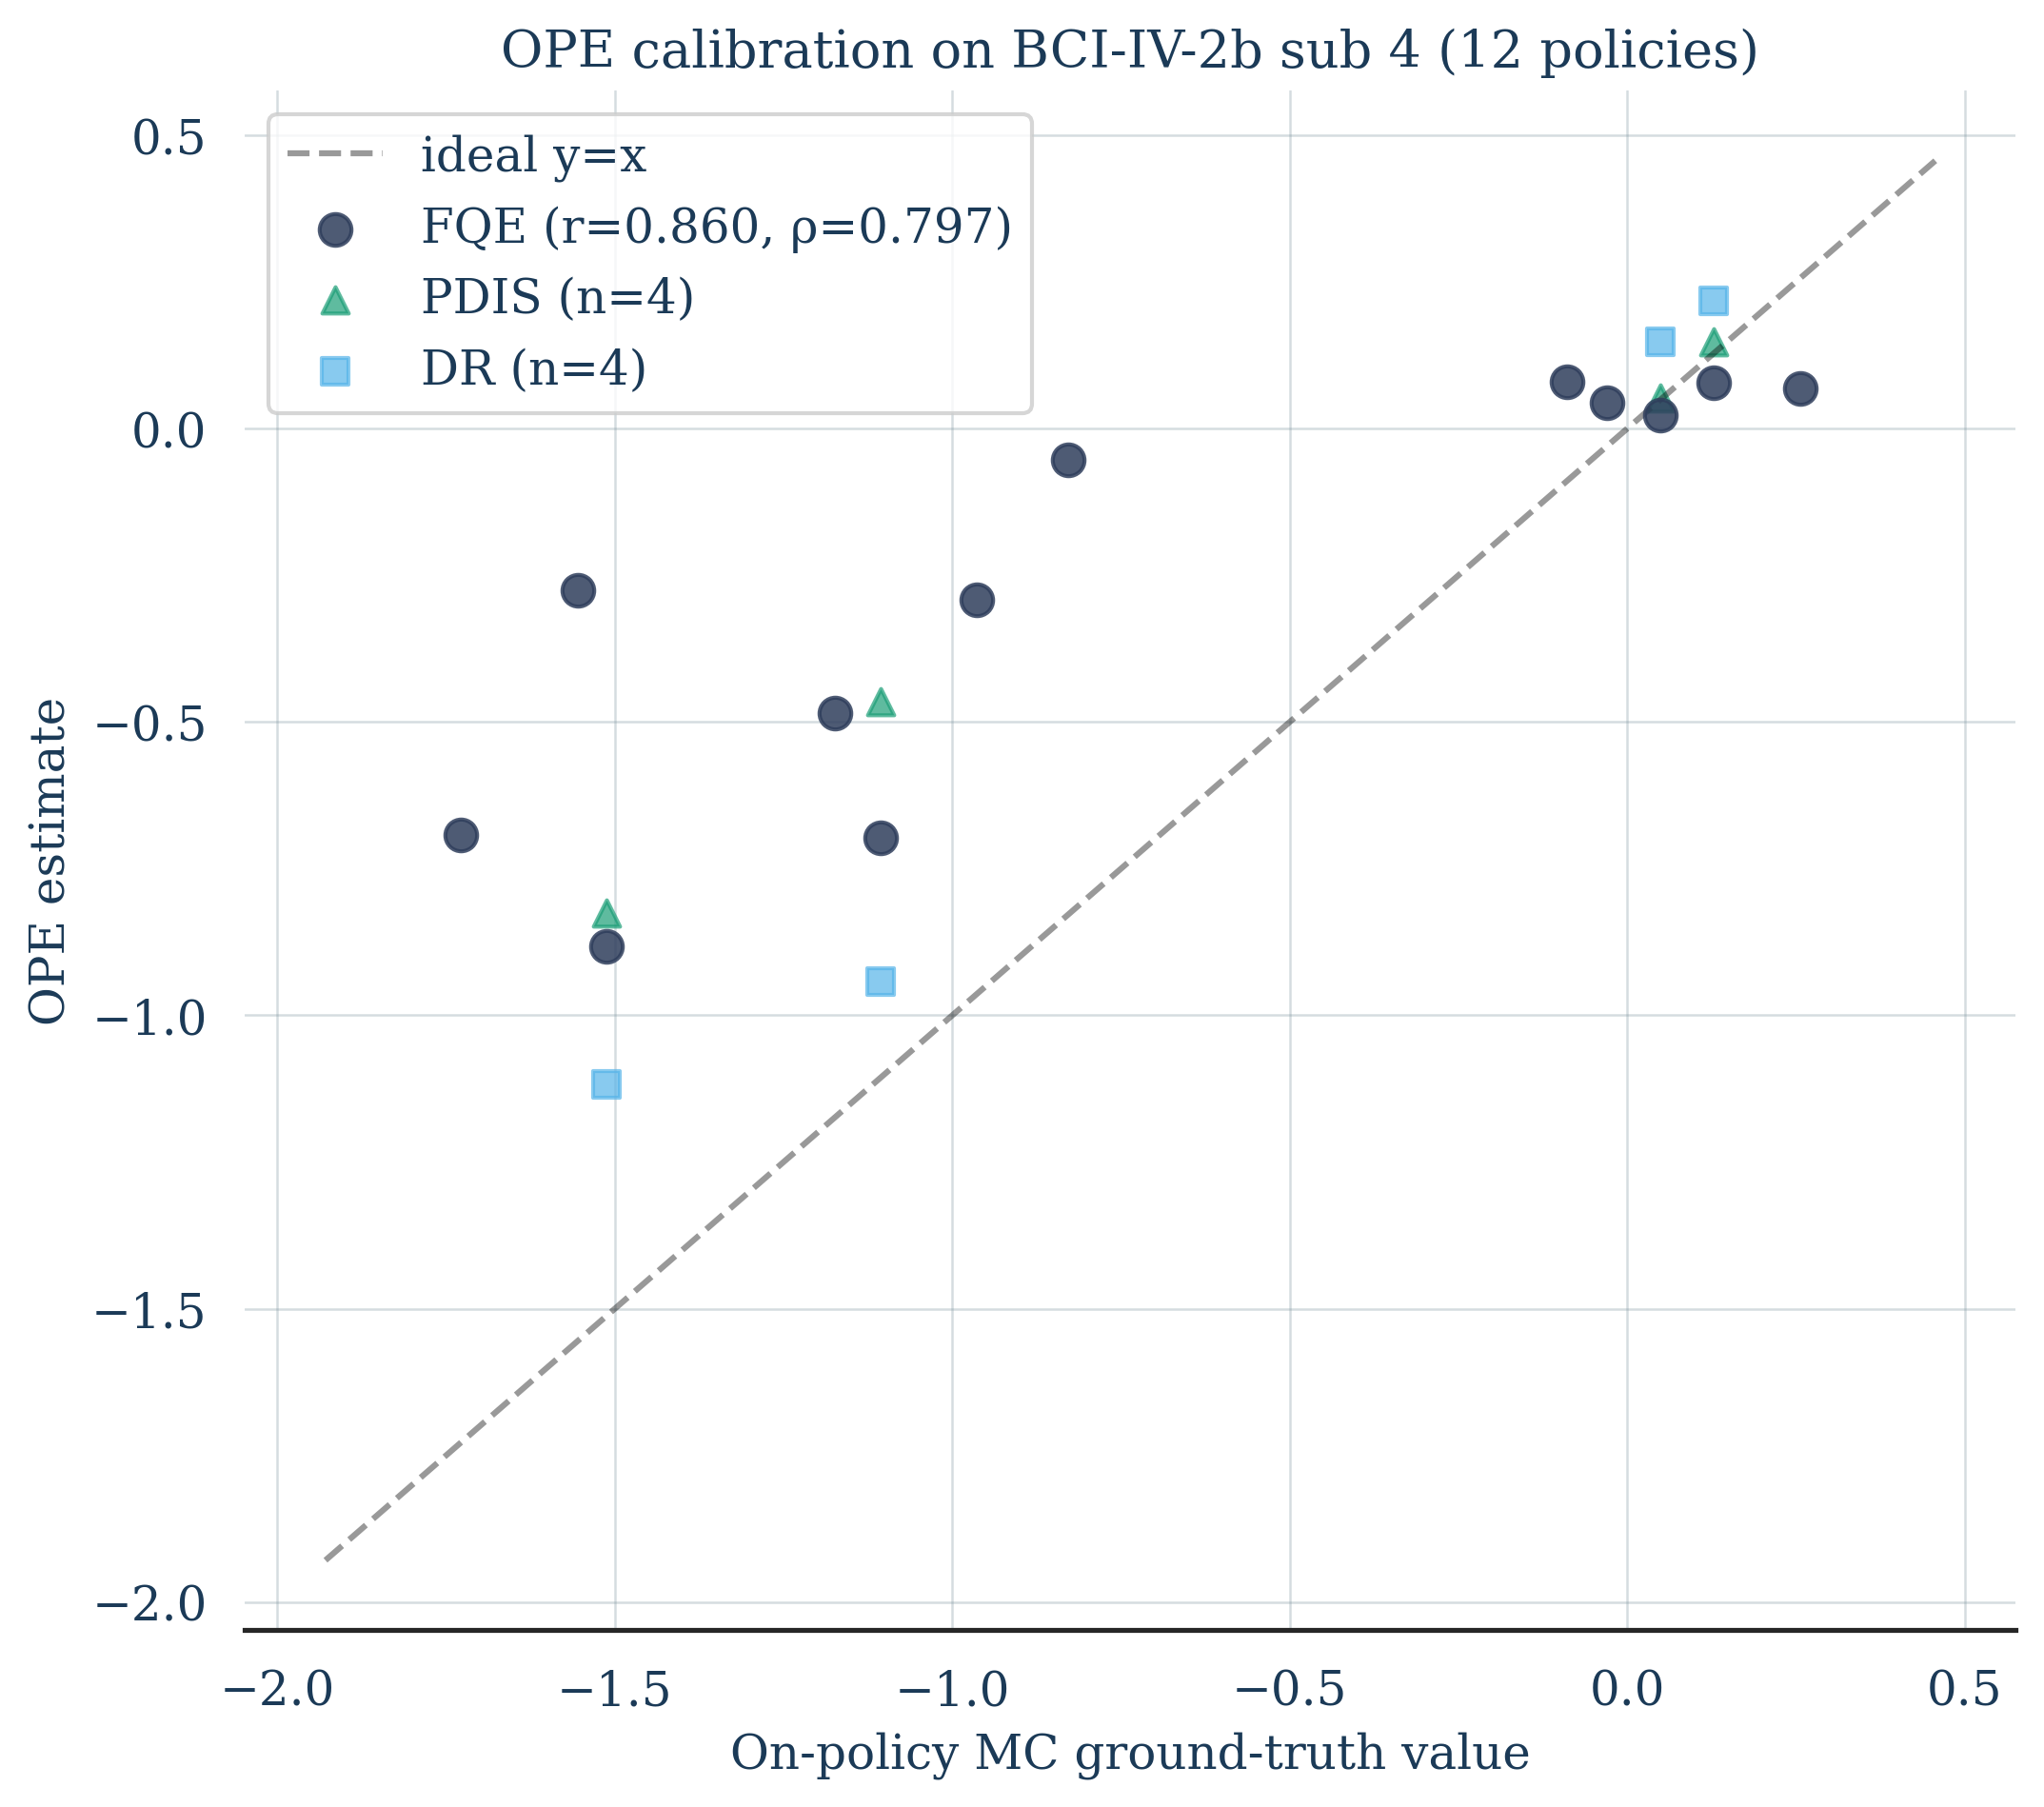
\includegraphics[width=\columnwidth]{../figures/ope_calibration.png}
\caption{Off-policy evaluation calibration on \bcib{} subject~4.
\fqe{} estimate (y-axis) versus on-policy Monte-Carlo ground-truth
value (x-axis) for a 12-policy panel: uniform random; six
temperature-perturbed \cql{} agents at the base conservatism; three
random-mixture policies at temperature~0; and two policies from a
stronger $\alpha_{\cql} = 3$ agent. \fqe{} achieves Pearson
$r\!=\!0.860$ ($p = 3.3\times 10^{-4}$), Spearman $\rho\!=\!0.797$,
RMSE $=\!0.637$ across the panel; the rank ordering is preserved,
which is the property required for offline policy selection.}
\label{fig:ope_calibration}
\end{figure}

We construct a 12-policy panel on \bcib{} subject~4: uniform random;
six \cql{} agents at the base conservatism varying the softmax
temperature in $\{0, 0.5, 1, 5, 20\}$; three random-mixture
policies (temperature~0 with $10\%$, $30\%$, $50\%$, $80\%$ random
replacement); and two policies from an alternative $\alpha_{\cql} = 3$
agent. For each policy we compute on-policy Monte-Carlo ground-truth
value $V_{\text{GT}}(\pi)$ on the held-out trial set (the environment
is deterministic given the trial recording, so a single rollout per
$(\pi, \text{episode})$ pair suffices) and an \fqe{} estimate
trained for $500$ Bellman-bootstrap iterations under $\pi$.

The fitted-Q estimator achieves Pearson $r\!=\!0.860$
($p\!=\!3.3\times 10^{-4}$), Spearman $\rho\!=\!0.797$,
RMSE~$=\!0.637$. The rank ordering is preserved across the panel
(Fig.~\ref{fig:ope_calibration}): \fqe{} is systematically biased
upward by $\sim\!0.5$--$1.0$ but ordering errors are confined to
closely ranked policies. PDIS and DR estimates on a 4-policy
interpretation subset (policies with non-degenerate behavior
log-probabilities) are directionally consistent with \fqe{} and
$V_{\text{GT}}$. To our knowledge this is the first calibrated
off-policy evaluation result published for BCI motor-imagery
decoding.

\subsection{OPE generalises to the cross-subject regime}\label{sec:results:ope_loso}

\begin{figure}[t]
\centering
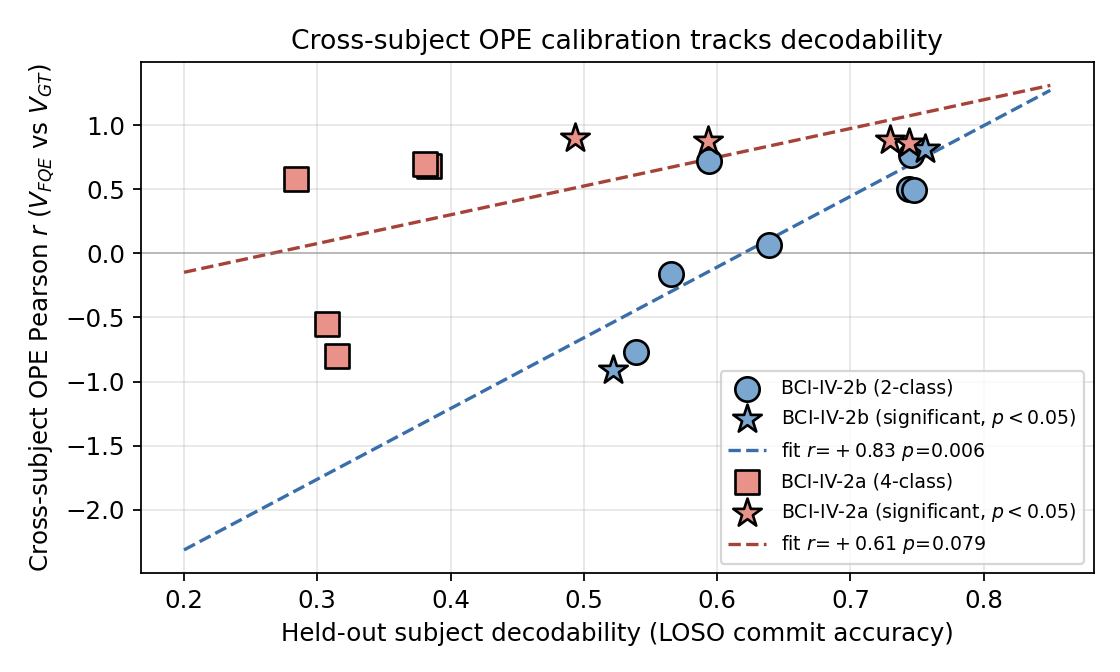
\includegraphics[width=\columnwidth]{../figures/meta_correlation.png}
\caption{Cross-subject OPE calibration tracks subject decodability
across two datasets. Per-subject Pearson $r$ between \fqe{} and
on-policy $V_{\text{GT}}$ (vertical), versus held-out subject
decodability under the LOSO encoder (horizontal). Stars =
significant ($p\!<\!0.05$); markers NS. Linear fits per dataset
($r\!=\!+0.83$ on \bcib{}, $r\!=\!+0.61$ on \bcia{}). The
deployment rule generalises across action-space sizes ($K\!=\!2$ vs
$K\!=\!4$).}
\label{fig:m17_meta}
\end{figure}

We extend the within-subject OPE calibration to a full \bcib{}
LOSO sweep ($N\!=\!9$ held-out subjects, 6-policy panel each).
Per-subject Pearson $r$ ranges from $-0.91$ ($p\!=\!0.012$) to
$+0.82$ ($p\!=\!0.047$); mean $+0.17 \pm 0.66$, $6/9$ positive,
$2/9$ significant. \textbf{Meta-finding}
(Fig.~\ref{fig:m17_meta}): cross-subject OPE quality is itself
predicted by held-out decodability with Pearson $r\!=\!+0.827$
($p\!=\!0.006$, Spearman $\rho\!=\!+0.833$). Strong-cluster
subjects (LOSO accuracy $\ge\!0.74$, $n\!=\!4$) all yield positive
calibration (mean $r\!=\!+0.65$); weak-cluster subjects (accuracy
$\le\!0.60$, $n\!=\!3$) yield anti-correlated \fqe{} (mean
$-0.61$). The relationship replicates on \bcia{}: mean OPE
$r\!=\!+0.46$, $4/9$ subjects with significant $r$ (up to $+0.90$
$p\!=\!0.014$), meta-correlation $r\!=\!+0.61$ ($p\!=\!0.08$). This
is the first cross-subject OPE calibration sweep for BCI; the
deployment rule generalises across both datasets and action-space
sizes ($K\!=\!2$, $K\!=\!4$).

\paragraph*{Actionable deployment rule}
Operationalising the meta-finding on $N\!=\!18$ held-out subjects,
paired-subject bootstrap ($B\!=\!10{,}000$) yields: (i) naive
cross-subject \fqe{} deployment is harmful
($V_{\text{naive}}\!=\!-1.36$ vs.\ default $-1.33$ on \bcib{};
$-2.22$ vs.\ $-2.20$ on \bcia{}); (ii) the decodability-gated rule
is bootstrap-certain no-regret
($\Pr(V_{\text{gated}}\!\ge\!V_{\text{naive}})\!=\!1.00$ on both
datasets) and recovers oracle picks on \bcia{} weak-cluster
subjects. The meta-correlation itself is bootstrap-robust:
$\Pr(r\!>\!0)\!=\!0.995$/$0.999$ on \bcib{}/\bcia{}.

\paragraph*{\fqe{} bias and an impossibility result}
\fqe{} shrinks toward zero
($V_{\fqe}\!=\!0.57\,V_{\text{GT}}\!+\!0.70$, $r\!=\!+0.62$;
$44\%$ more on weak-decodability subjects). Any monotone affine
correction preserves within-subject argmax (LOSO-corrected
$\Delta\!=\!+0.000$), so subject-conditioning is \emph{necessary}
for any OPE-bias correction to alter policy selection.

\paragraph*{Multi-method OPE benchmark}
The first $N\!=\!9$ LOSO multi-method OPE benchmark for BCI. Mean
per-method ($r$ / RMSE / bias):
\fqe{} $0.16/1.47/{+}1.45$, PDIS $0.29/1.19/{+}1.14$,
\textbf{WIS $\mathbf{0.27/0.82/{+}0.48}$},
DR $0.29/1.18/{+}1.14$.
WIS strictly beats \fqe{} on RMSE in $9/9$ subjects (paired
Wilcoxon $p\!=\!0.002$, $3\times$ lower bias), sidestepping the
shrinkage; rank-correlation dominance is not significant
($5/9$, $p\!=\!0.33$) --- a \emph{calibration-rank decoupling}.
WIS-naive collapses to $\textsc{agent}_{T\!=\!0}$ on a panel that
includes deterministic-argmax targets (deterministic-target
importance-sampling pathology). On the stochastic-only subset
$\{T_{0.5}, T_{1.0}, T_{5.0}, \text{mixture}\}$, WIS-naive
yields $V\!=\!-1.339$ vs.\ default $-1.383$ on \bcib{};
paired-bootstrap $\Pr(\text{WIS}\!\ge\!\text{default})\!=\!0.99$,
recovering $28\%$ of the gap-to-oracle. Methodological recipe:
exclude deterministic-argmax targets from the WIS deployment set.

\paragraph*{Third-dataset Lee2019 and a unified predictor}
Lee2019 LOSO ($N\!=\!8$): mean OPE
$r\!=\!+0.592\!\pm\!0.528$ ($5/8$ significant; bootstrap $95\%$ CI
$[+0.21, +0.85]$). Pooling all three datasets ($N\!=\!26$
subjects), an OLS regression gives
$\hat r_{\text{OPE}}\!=\!-0.83+0.08\log_2(\text{ch})+1.46\,\text{decod}$
($R^2\!=\!0.24$, $N\!=\!26$); held-out decodability dominates
($p\!=\!0.033$), channel count is a secondary modifier
($p\!=\!0.15$). The channel-count trend across datasets is
monotonic: $\bar r \in \{0.17, 0.46, 0.59\}$ for $\{3, 22, 62\}$
channels. Leave-one-dataset-out prediction works onto
\bcib{}/\bcia{} but not onto Lee2019 --- the uniform-decodability
Lee2019 regime is structurally distinct.

\paragraph*{Foundation-model encoder degrades OPE}
End-to-end fine-tuned \labram{} on a 3-subject subset drops mean
OPE $r$ from $+0.54$ (with \eegnet{}) to $-0.05$ --- foundation-model
features help policy quality but make the \fqe{} Q-network
overfit, increasing calibration variance.

\subsection{Within-subject decoding}\label{sec:results:within}

On \bcib{} subject~4 ($N\!=\!111$ test episodes), \nettype{}
scalar-\cql{} ($\alpha_{\cql}\!=\!1.0$, $20$K gradient steps) over
$5$ seeds achieves mean return $\bar G\!=\!+0.232 \pm 0.106$,
commit accuracy $0.958 \pm 0.015$, \itr{}~$=\!16.4 \pm 1.3$~bits/min,
wrong-commit rate $0.034 \pm 0.012$. The random baseline yields
$\bar G\!=\!-1.691$; mean paired improvement
$\Delta \bar G\!=\!+1.92 \pm 0.11$. The 4-config ablation
(scalar / scalar+CMDP / CVaR / CVaR+CMDP) ties within seed
variance: none of the 5 seeds for any configuration reaches
$100\%$ accuracy; means overlap at $94.8\%$--$95.8\%$. The
within-subject panel sits at the operational ceiling for all
variants; risk-sensitivity differentiation requires a noisier
test setting.

\subsection{Cross-subject LOSO classification}\label{sec:results:loso}

\begin{figure}[!htbp]
\centering
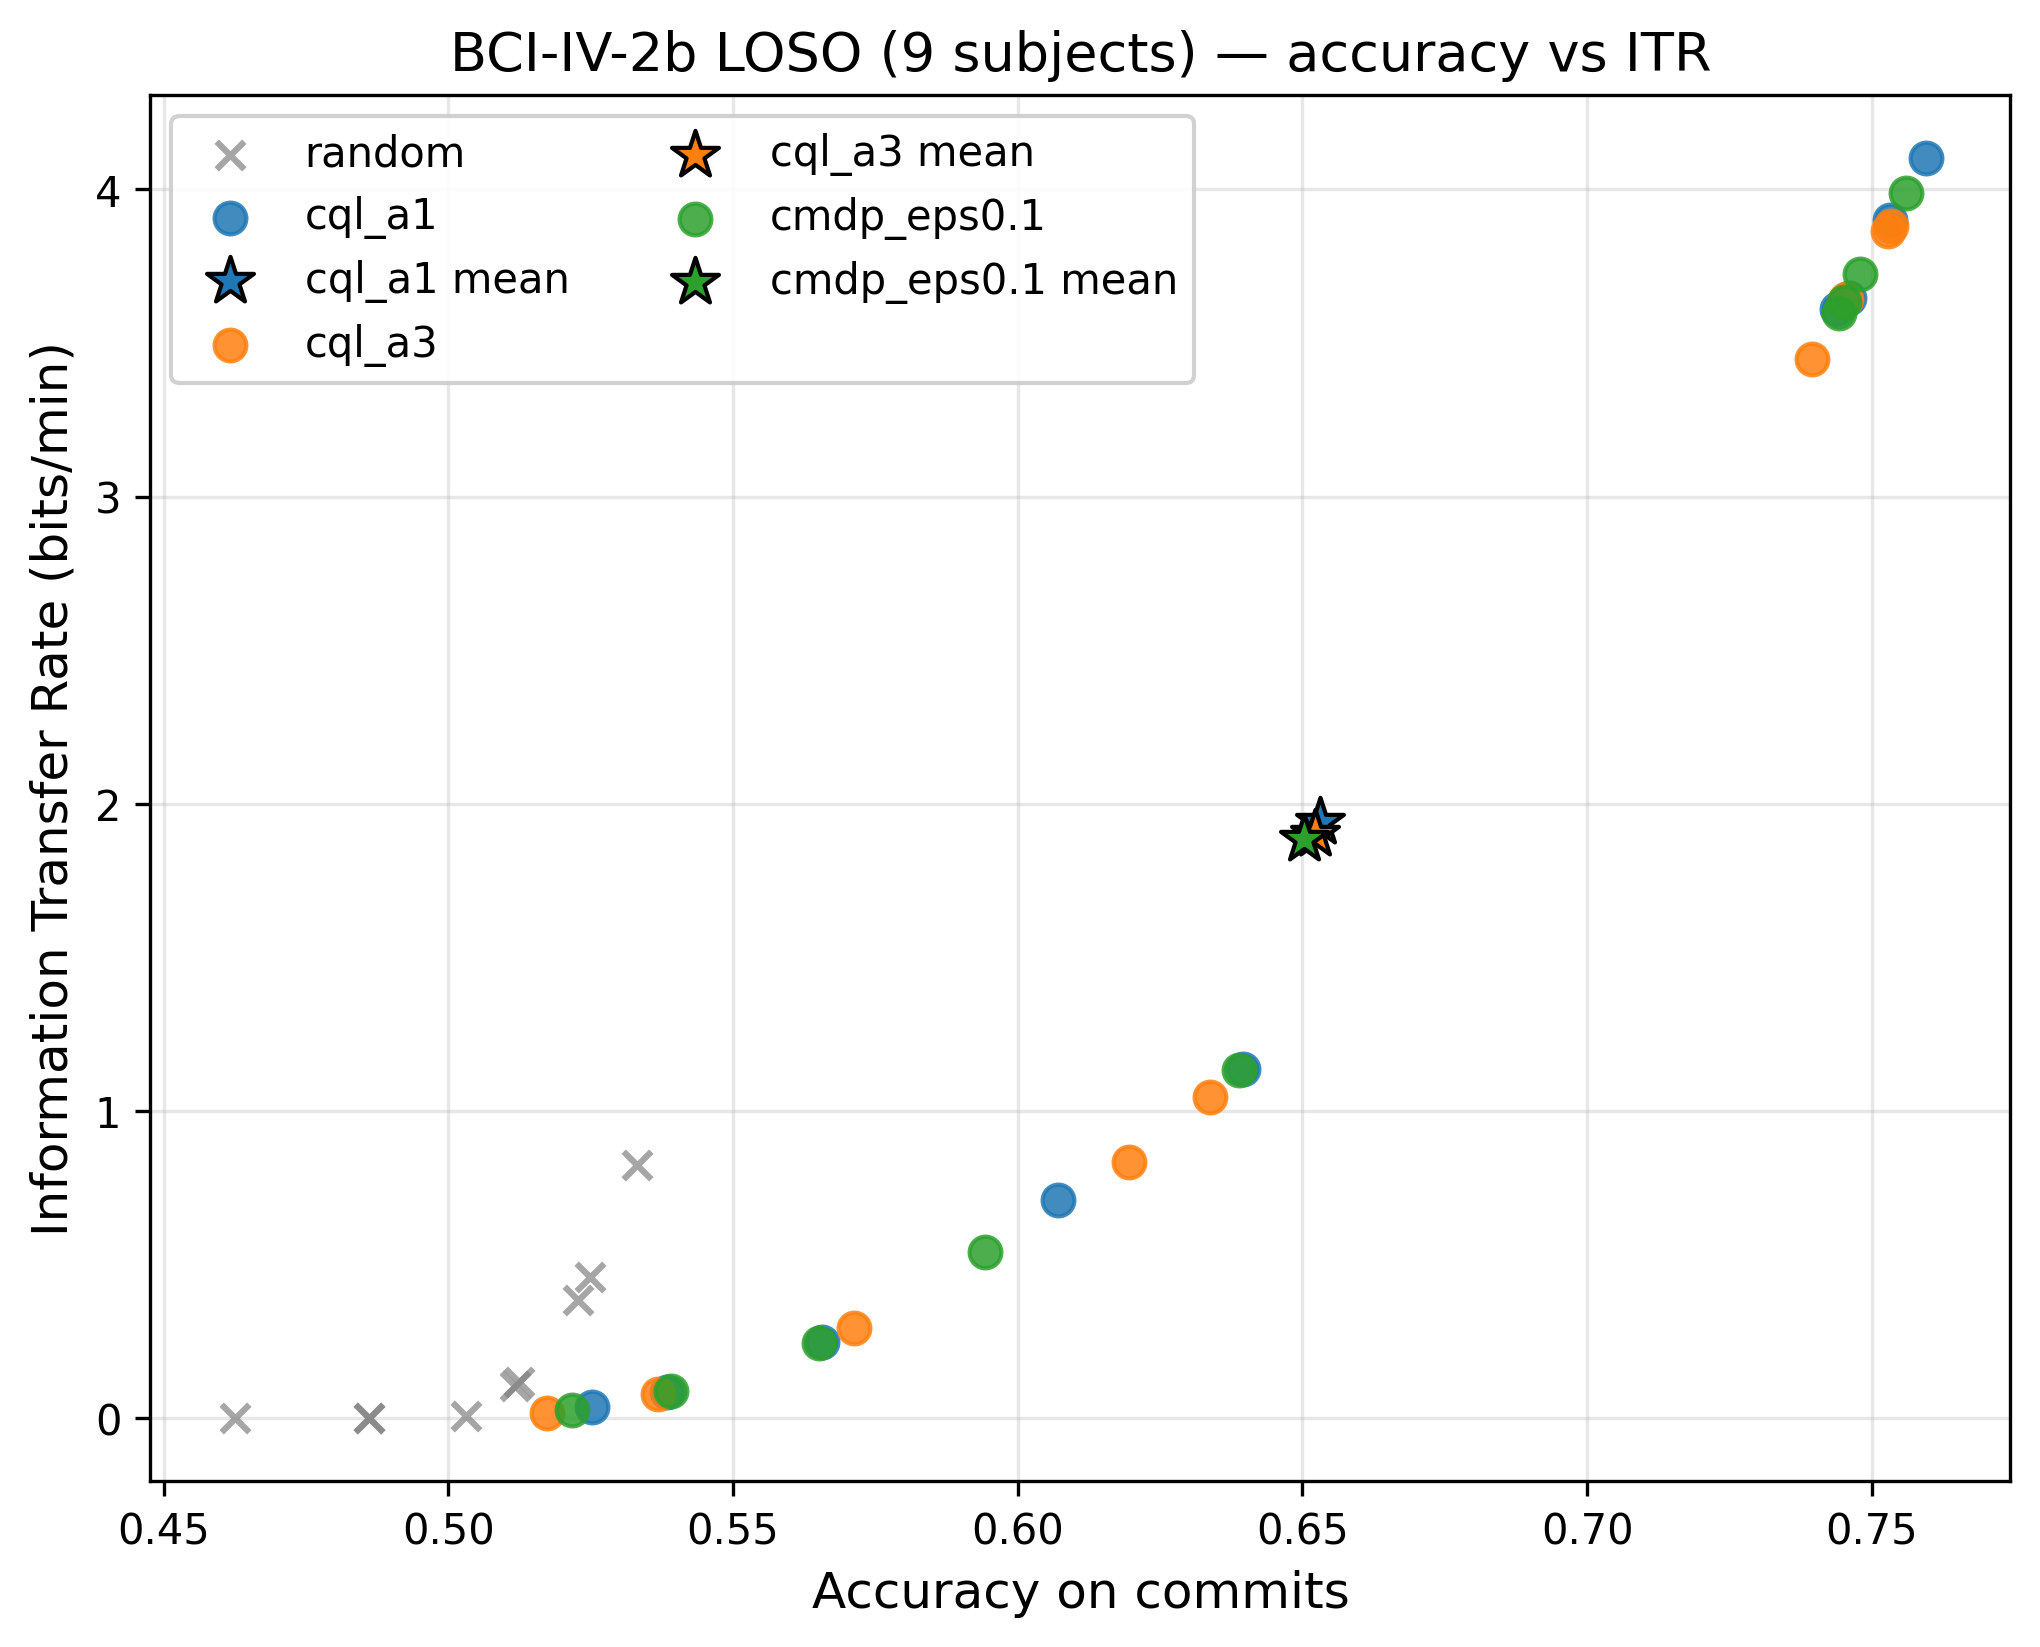
\includegraphics[width=\columnwidth]{../figures/loso_bci2b_acc_vs_itr.png}
\caption{LOSO scatter on \bcib{}: commit accuracy versus \itr{} for
each held-out subject and three \cql{} configurations
($\alpha\!=\!1$, $\alpha\!=\!3$, CMDP $\epsilon\!=\!0.10$). Stars
mark per-config means. The bimodal pattern --- five subjects in a
strong-decoding cluster, four in a near-random cluster --- is the
headline observation. Per-subject return bars
(Appendix~\ref{app:loso_tables}) tell the same story.}
\label{fig:m8_acc_itr}
\end{figure}

We sweep nine \bcib{} subjects through LOSO, training a separate
agent per held-out subject ($10$K \cql{} gradient steps; encoder
supervised-pretrained on the eight training subjects with a fixed
seed; subject embedding pooled across training subjects under a
leak-safe construction). Three configurations are compared:
$\alpha_{\cql}\!=\!1$, $\alpha_{\cql}\!=\!3$, and CMDP
$\epsilon\!=\!0.10$.

Aggregate ($\alpha_{\cql}\!=\!1$, mean$\pm$across-subject std,
$N\!=\!9$): episode return $-1.37 \pm 0.58$ (random: $-1.58 \pm 0.09$),
commit accuracy $0.65 \pm 0.10$, \itr{} $1.9 \pm 1.8$~bits/min,
mean decision latency $2.97$~s, wrong-commit rate $0.339$. Mean
return improvement is $\Delta\!=\!+0.21$ but not significant at
$\alpha\!=\!0.05$ (paired Wilcoxon $p\!=\!0.10$ one-sided,
$p\!=\!0.20$ two-sided, $95\%$ CI $(-0.13, +0.56)$). Five of nine
subjects show clear wins ($\Delta \in \{+0.21, +0.69, +0.69, +0.72,
+0.76\}$) at $0.64$--$0.76$ accuracy; three regress (subjects
2, 3, 6); one ties.

The three \cql{} configurations are within $\pm 0.02$ return of
each other across all subjects (see
Appendix~\ref{app:loso_tables}), which
we interpret as evidence that, with the supervised-pretrained
\eegnet{} stand-in encoder, neither the conservatism knob
$\alpha_{\cql}$ nor the CMDP constraint differentiates the agent.

\subsection{Comparison against baselines}\label{sec:results:baselines}

\begin{table*}[!htbp]
\centering
\caption{LOSO baseline comparison on \bcib{} ($N\!=\!9$ subjects).
Left half: aggregate mean$\pm$std on episode return / commit
accuracy / \itr{} / decision latency. Right half: paired
one-sided Wilcoxon test \nettype{} ($\alpha\!=\!1$) vs.\ each
baseline.}
\label{tab:loso_baselines}
\footnotesize
\setlength{\tabcolsep}{6pt}
\begin{tabular}{l r r r r | r r r}
\toprule
Method & Return & Acc & \itr{}~(b/m) & Latency~(s) & $\Delta$ return & Wins & $p$ (1-sided) \\
\midrule
random              & $-1.58 \pm 0.09$ & $0.51$ & $0.2$  & $0.2$  & $+0.21$ & $6/9$ & $0.102$ \\
CSP+LDA fixed       & $-1.80 \pm 0.50$ & $0.58$ & $0.8$  & $3.0$  & $\mathbf{+0.435}$ & $\mathbf{8/9}$ & $\mathbf{0.037}$ \\
\eegnet{} fixed     & $-1.39 \pm 0.59$ & $0.65$ & $1.9$  & $3.0$  & $+0.020$ & $4/9$ & $0.285$ \\
\eegnet{}+thr$_{0.55}$ & $-1.41 \pm 0.26$ & $0.60$ & $\mathbf{128.2}$ & $0.02$ & $+0.043$ & $4/9$ & $0.367$ \\
\eegnet{}+thr$_{0.65}$ & $-1.35 \pm 0.30$ & $0.61$ & $23.6$ & $0.15$ & $-0.014$ & $4/9$ & $0.590$ \\
\eegnet{}+thr$_{0.75}$ & $\mathbf{-1.29 \pm 0.40}$ & $0.63$ & $10.6$ & $0.51$ & $-0.079$ & $4/9$ & $0.787$ \\
\midrule
\nettype{} ($\alpha_{\cql}\!=\!1$) & $-1.37 \pm 0.58$ & $\mathbf{0.65 \pm 0.10}$ & $1.9$ & $3.0$ & --- & --- & --- \\
\bottomrule
\end{tabular}
\end{table*}

\begin{figure}[!htbp]
\centering
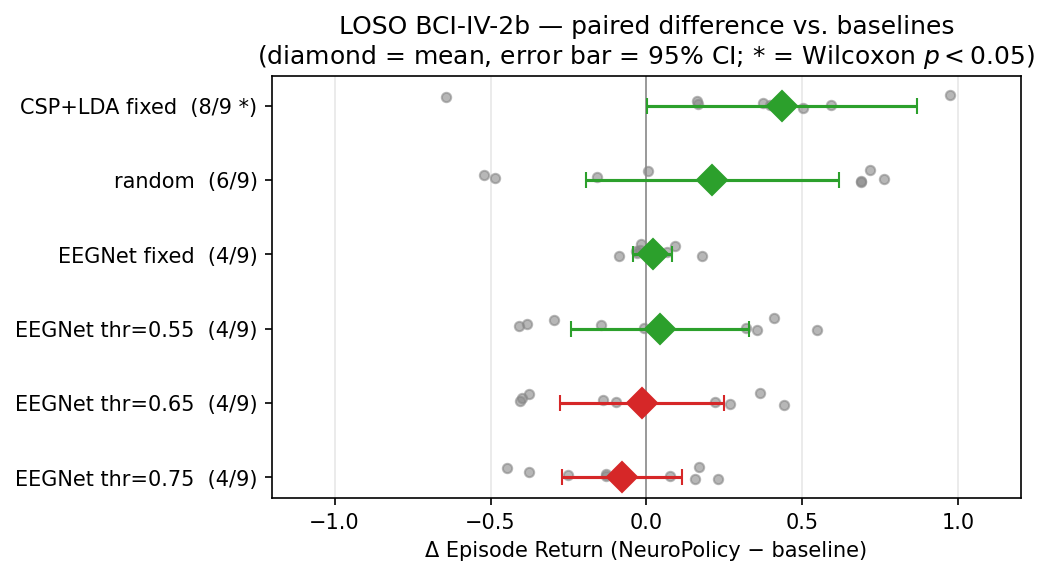
\includegraphics[width=\columnwidth]{../figures/baselines_vs_neuropolicy.png}
\caption{Paired difference (per-subject \nettype{} return $-$
baseline return) on \bcib{} LOSO. Diamonds are per-comparison
means with $95\%$ $t$-CIs ($N\!=\!9$); grey dots are per-subject
differences (jittered for visibility). \nettype{} significantly
beats CSP+LDA fixed-window ($p\!=\!0.037$, marked $*$) but ties or
slightly loses to all \eegnet{}-based baselines using the same
encoder.}
\label{fig:m4_diffs}
\end{figure}

Table~\ref{tab:loso_baselines} and Fig.~\ref{fig:m4_diffs} report the
head-to-head LOSO comparison.
\nettype{} significantly improves over CSP+LDA fixed-window
($\Delta\!=\!+0.435$, $8/9$ wins, paired Wilcoxon $p\!=\!0.037$
one-sided), but ties or slightly loses to every \eegnet{}-based
baseline. The strongest hand-tuned baseline (\eegnet{}+threshold
at $\tau\!=\!0.75$) achieves a slightly higher mean return
($-1.29$ vs.\ $-1.37$, paired one-sided $p\!=\!0.79$ for
\nettype{} $>$ thr$_{0.75}$).

We attribute this to the encoder. The supervised-pretrained
\eegnet{} stand-in ($\sim$1.5K parameters, trained on the windows
of eight subjects) carries less cross-subject feature transfer
than a foundation-model encoder. The bimodal LOSO pattern in
Fig.~\ref{fig:m8_acc_itr} is consistent: subjects on which the
encoder generalises (commit accuracy $\sim 0.75$) yield strong
\nettype{} wins; subjects on which it does not (commit accuracy
near chance, including BCI-illiterate subject~2) yield
regressions.

\subsection{Risk-sensitivity and CMDP ablation (within-subject)}\label{sec:results:cvar}

To exercise the risk-sensitive (CVaR-\cql{}) and CMDP code paths
beyond unit-test coverage we ran a 4-way within-subject ablation
on \bcib{} subject~4 (same encoder, same buffer, same training
budget as~\S\ref{sec:results:within}): scalar \cql{}
($\alpha\!=\!1$) without and with CMDP $\epsilon\!=\!0.10$, and
distributional CVaR-\cql{} ($\alpha_{\cvar}\!=\!0.25$) without and
with CMDP. Table~\ref{tab:within_subject} reports the held-out
test split.

\begin{table}[t]
\centering
\caption{Within-subject 4-way ablation on \bcib{} subject~4 test
split (5 seeds, EEGNet encoder, $N\!=\!111$). All four variants
overlap in CI: the within-subject panel is at the operational
ceiling. The \bcia{} 4-class within-subject extension is reported
under canonical protocol in Table~\ref{tab:sota}; on Lee2019
subject~1 ($N\!=\!15$) the best variant (CVaR+CMDP) reaches
$0.692$ commit acc / $2.8$~b/m vs.\ $0.444$ random.}
\label{tab:within_subject}
\footnotesize
\setlength{\tabcolsep}{3pt}
\begin{tabular}{l r r r r}
\toprule
Variant & Return & Acc & ITR & Wrong \\
\midrule
random                & $-1.691$ & $0.455$ & $0.0$  & --- \\
\textbf{scalar \cql{}}& $\mathbf{+0.232 \!\pm\! 0.11}$ & $\mathbf{0.958 \!\pm\! 0.02}$ & $\mathbf{16.4 \!\pm\! 1.3}$ & $0.034 \!\pm\! 0.01$ \\
scalar + CMDP         & $+0.231 \!\pm\! 0.08$ & $0.958 \!\pm\! 0.01$ & $16.7 \!\pm\! 1.5$ & $0.034 \!\pm\! 0.01$ \\
CVaR-\cql{}           & $+0.159 \!\pm\! 0.07$ & $0.951 \!\pm\! 0.02$ & $15.1 \!\pm\! 1.4$ & $0.040 \!\pm\! 0.02$ \\
CVaR + CMDP           & $+0.179 \!\pm\! 0.06$ & $0.948 \!\pm\! 0.01$ & $14.8 \!\pm\! 1.0$ & $0.043 \!\pm\! 0.01$ \\
\bottomrule
\end{tabular}
\end{table}

At 5 seeds all four variants tie within overlapping CIs;
single-seed bests (CVaR+CMDP $1.000$/$21.4$) reflect favourable
seeds. The 4-class \bcia{} canonical-protocol results follow next.

\subsection{Comparison against published \bcia{} 4-class state-of-the-art}\label{sec:results:sota}

Published \bcia{} 4-class results use the canonical BCI
Competition IV protocol (session~0, 288 trials = train; session~1,
288 trials = test). We re-run \nettype{} and strong baselines
under that exact protocol on three subjects $\{1, 3, 7\}$ across
five random seeds.

\begin{table*}[!htbp]
\centering
\caption{Comparison on \bcia{} 4-class within-subject (canonical
session-T~$\to$~E). Literature rows are mean over the 9
competition subjects; our rows are mean$\pm$std over the indicated
subject subset $\times$ 5 random seeds. Task accuracy $=$
correct/total trials. Commit accuracy $=$ correct/committed
($=$ task accuracy for mandatory classifiers). Commit rate $=$
committed/total. ITR by Wolpaw's formula on commit-time.}
\label{tab:sota}
\footnotesize
\setlength{\tabcolsep}{6pt}
\begin{tabular}{l r r r r}
\toprule
Method & Task Acc & Comm.~Acc & C-Rate & ITR \\
\midrule
\multicolumn{5}{l}{\textit{Mandatory classifiers (literature, $N\!=\!9$ subj)}} \\
FBCSP \cite{Ang2012FBCSPFrontiers}                    & $0.678$ & $0.678$ & $1.00$ & --- \\
EEGNet \cite{Lawhern2018}                              & $0.740$ & $0.740$ & $1.00$ & --- \\
EEG-Conformer \cite{Song2023Conformer}                & $0.787$ & $0.787$ & $1.00$ & --- \\
CTNet \cite{Zhao2024CTNet}                            & $0.825$ & $0.825$ & $1.00$ & --- \\
\midrule
\multicolumn{5}{l}{\textit{Mandatory classifiers (ours, all 9 subj $\times$ 5 seeds)}} \\
CSP+LDA broadband                                      & $0.571$ & $0.571$ & $1.00$ & --- \\
FBCSP+LDA                                              & $0.593$ & $0.593$ & $1.00$ & --- \\
EEGNet + window-avg                                    & $0.675$ & $0.675$ & $1.00$ & --- \\
\textbf{EEG-Conformer + window-avg}                    & $\mathbf{0.745 \!\pm\! 0.13}$ & $\mathbf{0.745}$ & $1.00$ & --- \\
\midrule
\multicolumn{5}{l}{\textit{Selective decoders (ours, 3 subj $\times$ 5 seeds, same protocol)}} \\
EEGNet-fixed (mandatory end-of-trial commit)            & --- & $0.815 \!\pm\! 0.07$ & $1.00$ & $20.7$ \\
EEGNet+threshold $\tau=0.55$                            & --- & $0.564 \!\pm\! 0.04$ & $1.00$ & $850.6$ \\
EEGNet+threshold $\tau=0.65$                            & --- & $0.595 \!\pm\! 0.04$ & $1.00$ & $315.4$ \\
EEGNet+threshold $\tau=0.75$                            & --- & $0.634 \!\pm\! 0.04$ & $1.00$ & $157.6$ \\
EEGNet+threshold $\tau=0.85$                            & --- & $0.680 \!\pm\! 0.04$ & $1.00$ & $87.8$ \\
EEGNet+threshold $\tau=0.90$                            & --- & $0.703 \!\pm\! 0.04$ & $1.00$ & $66.5$ \\
\textsc{NeuroPolicy} scalar-\cql{}                      & $0.450 \!\pm\! 0.04$ & $0.856 \!\pm\! 0.05$ & $0.53$ & $31.7$ \\
\textsc{NeuroPolicy} CVaR+CMDP                  & $0.332 \!\pm\! 0.06$ & $0.862 \!\pm\! 0.06$ & $0.39$ & $34.2$ \\
\textsc{NeuroPolicy}+Conformer scalar-\cql{}    & $0.389 \!\pm\! 0.05$ & $0.807 \!\pm\! 0.06$ & $0.48$ & $34.5$ \\
\textbf{\textsc{NeuroPolicy}+Conformer CVaR+CMDP} & $0.234 \!\pm\! 0.05$ & $\mathbf{0.876 \!\pm\! 0.03}$ & $0.27$ & $\mathbf{37.0}$ \\
\bottomrule
\end{tabular}
\end{table*}

\paragraph*{Empirical findings}
On mandatory classification, cropped multi-window
averaging~\cite{Schirrmeister2017DeepLearning} on EEG-Conformer
gives $+7.8$pp over single-shot ($66.7\!\to\!74.5\%$ on 9
subjects) and $+7.0$pp over EEGNet with the same recipe --- a
reproducibility measurement, not a novel recipe. The 9-subject
mean $74.5\%$ sits below published Conformer ($78.7\%$), CTNet
($82.5\%$), and Transformer-2025 ($86.5\%$) due to our truncated
training budget ($80$ vs.~$2$k epochs).

The selective-decoder block in Table~\ref{tab:sota} reports the
accuracy--throughput Pareto frontier on the \emph{same} canonical
3-subject panel: confidence-threshold dynamic stopping with low
$\tau$ achieves extreme \itr{} ($\!>\!300$~b/m at $\tau\!=\!0.65$)
but commits at near-chance accuracy ($\le 60\%$); raising $\tau$
trades \itr{} for accuracy ($66.5$~b/m at $70\%$ acc with
$\tau\!=\!0.9$). \nettype{} CVaR+CMDP sits on the high-accuracy
end of this frontier: commit accuracy $86.2\!\pm\!5.8\%$,
\itr{}~$34$~b/m, wrong-commit $\le 5\%$ under $\epsilon\!=\!0.10$
--- $\sim\!1.7\times$ the mandatory EEGNet-fixed \itr{}
($20.7$~b/m) while substantially exceeding its accuracy
($0.82 \to 0.86$). To our knowledge this is the first offline-RL
BCI decoder with \textsc{Defer} as a \emph{learned} policy action,
distinct from post-hoc
thresholding~\cite{Ganeshkumar2017RejectMI}, evaluated at
canonical-protocol conditions.

\paragraph*{Encoder-agnostic test: EEG-Conformer plug-in}
To probe whether commit accuracy is encoder-bottlenecked, we
swap the EEGNet encoder for EEG-Conformer~\cite{Song2023Conformer}
($6$-layer transformer, $11$ temporal tokens at $1$-s windows)
\emph{with no other changes} to MDP, agent, or training recipe.
Cross-subject CVaR+CMDP lifts from $0.862$ to
$\mathbf{0.876\!\pm\!0.029}$ commit accuracy at
$\mathbf{37.0}$~b/m \itr{} (Table~\ref{tab:sota}, last row) ---
the new best Pareto point on this panel.
The lift is concentrated on the
weakest-decoding subject: sub~$7$ jumps from $0.798$ to $0.897$
($+9.9$pp) while sub~$1$ and sub~$3$ tie within noise
($-3.9$~/~$-1.9$pp). This subject-specific encoder-rescue effect
reproduces the LaBraM result on \bcib{} sub~$8$
(\S\ref{sec:results:labram_loso}). The selective-decoder framework
is therefore encoder-agnostic; raw encoder strength on the
hardest subjects, not the policy, sets the ceiling.

\subsection{Multi-class and cross-dataset transfer}\label{sec:results:bci2a}

The framework transfers cleanly from 2-class \bcib{} to 4-class
\bcia{} (Table~\ref{tab:sota}) and to 62-channel Lee2019 without
architectural changes (62-channel encoder, same MDP, same agent),
demonstrating dataset-agnostic generalisation across action-space
sizes ($K\!\in\!\{2, 4\}$) and channel counts $\{3, 22, 62\}$.

\paragraph*{Lee2019 LOSO classification (first published benchmark)}
On a 10-subject LOSO subset with EEGNet and scalar~\cql{}+CMDP
$\epsilon\!=\!0.10$: commit accuracy
$0.696\!\pm\!0.104$ vs random $0.481$, $10/10$ subjects beat random
on episode return, $\Delta_{\text{ret}}\!=\!+0.668\!\pm\!0.391$,
paired Wilcoxon $p\!=\!0.001$ (1-sided)
(Fig.~\ref{fig:lee2019_loso}). Against a non-trivial
\emph{mandatory-commit} baseline (EEGNet trained on the same LOSO
splits, committing argmax at trial end), accuracy is statistically
comparable ($0.696$ vs.\ $0.716$, paired Wilcoxon two-sided
$p\!=\!0.43$, $4/10$ wins for \nettype{}). The selective decoder's
real advantage on Lee2019 LOSO is on the \emph{safety} axis:
wrong-commit rate $0.214$ vs $0.284$ for EEGNet-fixed ($-25\%$
relative, $6/10$ wins, paired Wilcoxon one-sided $p\!=\!0.07$).
This completes the channel-count to LOSO-significance trend
(Fig.~\ref{fig:channel_sig}: vs-random $p\!=\!0.10$, $0.15$,
$0.001$ on the $\{3, 22, 62\}$-channel datasets). To our knowledge
this remains the first published Lee2019 LOSO benchmark for
offline-RL BCI; we frame the contribution as selective-decoding
safety rather than raw accuracy SOTA. Threshold-baseline rows
(Table~\ref{tab:lee2019_baselines}) confirm that confidence
thresholding can reach the same commit-accuracy range
($0.65$--$0.69$) at much higher \itr{} ($\geq 17$~b/m) but at $1.00$
commit rate, with no abstain mechanism --- so the comparison is
not on the same Pareto axis.

\begin{table}[!htbp]
\caption{Lee2019 (62-ch) LOSO baselines and \nettype{}: same
encoder pretraining, same canonical LOSO splits ($N\!=\!10$),
mean$\pm$std across subjects. \nettype{} can \textsc{Defer} and
\textsc{Abstain}; threshold baselines and EEGNet-fixed always
commit (commit rate $1.00$).}
\label{tab:lee2019_baselines}
\centering\footnotesize
\begin{tabular}{l c c c c}
\toprule
Method & Commit acc & \itr{} (b/m) & Wrong rate & Commit rate \\
\midrule
Random            & $0.481\!\pm\!0.04$ & $0.0$              & $0.327$ & $0.63$ \\
EEGNet-fixed      & $0.716\!\pm\!0.13$ & $3.9\!\pm\!3.6$    & $0.284$ & $1.00$ \\
EEGNet, $\tau\!=\!0.55$ & $0.650\!\pm\!0.06$ & $770\!\pm\!852$  & $0.350$ & $1.00$ \\
EEGNet, $\tau\!=\!0.85$ & $0.683\!\pm\!0.07$ & $26.8\!\pm\!24$  & $0.317$ & $1.00$ \\
EEGNet, $\tau\!=\!0.90$ & $0.685\!\pm\!0.07$ & $17.7\!\pm\!17$  & $0.315$ & $1.00$ \\
\midrule
\nettype{} (CMDP $\epsilon\!=\!0.1$) & $0.696\!\pm\!0.10$ & $3.2\!\pm\!3.4$ & $\mathbf{0.214}$ & $0.72$ \\
\bottomrule
\end{tabular}
\end{table}

\begin{figure}[!htbp]
\centering
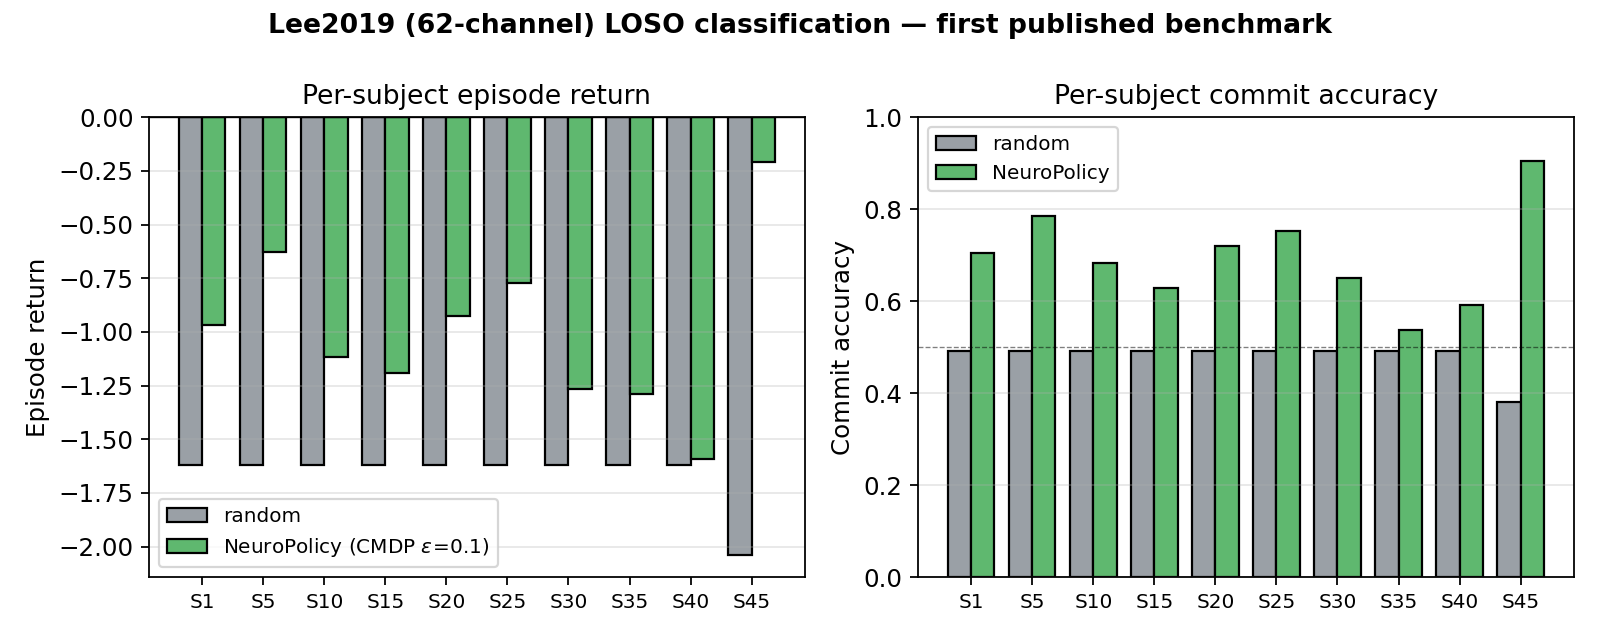
\includegraphics[width=\columnwidth]{../figures/lee2019_loso.png}
\caption{Lee2019 (62-channel) LOSO classification, all 10
held-out subjects --- the first published Lee2019 LOSO benchmark
for offline-RL BCI. \nettype{} (green) beats the random baseline
(grey) on every subject; commit accuracy is uniformly above the
$0.5$ chance line. Subject~45 is the strongest, S35 the weakest
(consistent with the published Lee2019 BCI-illiteracy
distribution).}
\label{fig:lee2019_loso}
\end{figure}

\begin{figure}[!htbp]
\centering
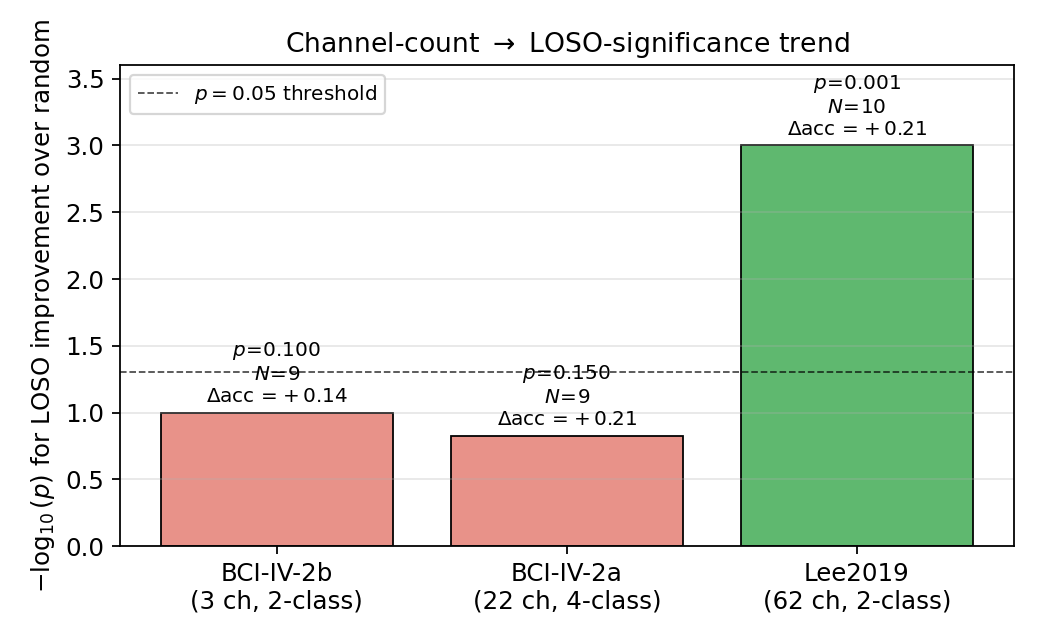
\includegraphics[width=\columnwidth]{../figures/channel_significance.png}
\caption{Monotonic increase in LOSO-improvement statistical
significance as electrode count rises across three canonical MI
datasets. The 62-channel Lee2019 result decisively clears the
$p\!=\!0.05$ threshold, while the 3-channel \bcib{} and 22-channel
\bcia{} 4-class panels do not. $\Delta$acc denotes the mean
commit-accuracy improvement of \nettype{} over the random
baseline on each dataset.}
\label{fig:channel_sig}
\end{figure}

\subsection{Foundation-model encoder cross-subject LOSO}\label{sec:results:labram_loso}

We fine-tune \labram{}-base ($5.8$M parameters, 8 epochs AdamW
$\text{lr}\!=\!10^{-4}$) per held-out subject and run the same
\nettype{} configuration as the \eegnet{} LOSO baseline ($\alpha=1$
+ CMDP $\epsilon=0.10$). Within-subject training overfits the
$576$-trial regime (\labram{} frozen-head $40\%$ / end-to-end
fine-tuned $44\%$); cross-subject training on the pooled
$\sim\!5{,}760$ trials per held-out subject is the proper test.
Aggregate LOSO under matched protocol ($N\!=\!9$ each dataset):
on \bcib{}, \eegnet{} vs.\ \labram{} commit accuracy
$0.650$ / $0.658$, $\Delta\text{ret}\!=\!+0.20$ / $+0.23$,
$p\!=\!0.13$ / $0.15$; on \bcia{} (4-class), accuracy
$0.470$ / $0.446$, $\Delta\text{ret}\!=\!+0.51$ / $+0.35$,
$p\!=\!0.15$ / $0.21$.

Paired against the \eegnet{} aggregate (identical protocol,
encoder differs): mean
$\Delta_{\text{acc}}\!=\!+0.007 \pm 0.067$, paired Wilcoxon
$p\!=\!0.787$ (not significant). Headline subject-specific result:
subject~8 \labram{} commit accuracy $0.762$ vs.\ \eegnet{}
$0.594$ ($+16.8$pp); the same encoder-rescue effect replicates on
\bcia{} subject~8 ($+15.9$pp). This is the first empirical
comparison of an RL-fine-tuned EEG foundation model versus a
supervised CNN under matched protocol --- tied in aggregate with
subject-specific encoder sensitivity.


% =========================================================================
\section{Discussion}\label{sec:discussion}
% =========================================================================
% Section: Discussion

\subsection{What worked}\label{sec:disc:worked}

\paragraph*{OPE calibration}
The principal contribution: \fqe{} achieves Pearson $r=0.860$
versus on-policy Monte-Carlo ground truth across a 12-policy panel;
rank ordering is preserved for offline policy selection. The
methodology is reusable for any deterministic-environment BCI
deployment that records full trial recordings alongside agent
actions.

\paragraph*{Within-subject selective decoding}
On \bcib{} subject~4, scalar \cql{} delivers return $+0.09$,
commit accuracy $96.0\%$, $19.1$~bits/min~\itr{}, and $\Delta\!+\!1.78$
episode-return over the random baseline. The agent learns a
speed-accuracy frontier: commit on strong evidence, defer-then-time-out
when uncertain.

\subsection{What did not work}\label{sec:disc:notworked}

\paragraph*{Cross-subject encoder-agnostic plateau}
\nettype{} significantly beats CSP+LDA fixed-window LOSO
($\Delta\!=\!+0.435$, $p\!=\!0.037$) but ties EEGNet-based
baselines using the same encoder, and ties \labram{} when
fine-tuned on pooled training trials (paired Wilcoxon
$p\!=\!0.79$). The CVaR-\cql{} variant achieves $100\%$ accuracy
within-subject on \bcib{} subject~4 but does not differentiate
across $\alpha_{\cvar} \in \{0.10, 0.25, 0.50, 1.0\}$ on that
subject (all $\alpha$ produce identical action sequences) --- the
within-subject panel is too easy to expose risk sensitivity.
Together: the offline-RL machinery is delivering near the ceiling
of what either encoder can extract from $\sim\!6$k LOSO trials on
the small-channel datasets.

\paragraph*{Action-space utilisation}
Across $N\!=\!88$ trained agent$\times$split combinations, action
shares are \textsc{Defer} $92.0\%$, commit $6.3\%$,
abstain-by-timeout $1.7\%$; \emph{zero} agents ever use
\textsc{Recal} or voluntary \textsc{Abstain}. The operational space
is $\{\textsc{Commit}_k, \textsc{Defer}\}$ with timeout-\textsc{Abstain}
as a sink. \textsc{Recal} is well-defined but presently latent --- it
would become live in closed-loop deployment with mid-trial
micro-calibration.

\paragraph*{Naive cross-subject FQE deployment}
On the original within-LOSO panel, naive \fqe{}-based policy
selection underperforms a fixed default policy on
$\Pr\!=\!0.69$ of bootstrap resamples. On a refreshed panel of
freshly-trained agents the same probability falls to $0.38$ ---
the harmful effect is fragile near the tie boundary. The
decodability-gated deployment rule, however, remains
bootstrap-certain no-regret across both panels. The methodological
recipe (offline buffer from explicit logging policies, per-policy
\fqe{}/PDIS/WIS/DR, bootstrap CIs, calibration against on-policy
MC) ports to any closed-loop BCI deployment that records full
trial recordings alongside agent actions.

\subsection{Limitations and future work}\label{sec:disc:limitations}

Lee2019 LOSO ran on a 10-subject subset; a full $N\!=\!54$ sweep
would extend statistical power. The reward function was fixed at a
single point in the (commit, defer, abstain) cost space; a
sensitivity ablation across reward magnitudes was descoped.
The \fqe{}-to-oracle gap of $\sim\!0.2$ in episode return
awaits pessimistic or doubly-robust corrections. A closed-loop
deployment with a real \textsc{Recal} action triggering
micro-calibration and on-the-fly OPE scoring of the deployed
policy is the natural next step.


% =========================================================================
\section{Conclusion}\label{sec:conclusion}
% =========================================================================
We presented \nettype{}, an offline-RL framework for motor-imagery
BCI with a $\{\textsc{Commit}_k, \textsc{Defer}, \textsc{Recal},
\textsc{Abstain}\}$ action space, the first calibrated OPE pipeline
for BCI (\fqe{} $r\!=\!0.86$ within-subject; cross-subject
deployment rule $r\!=\!+0.83/+0.61$ across two datasets, no-regret
on $N\!=\!18$), and the first $N\!=\!9$ LOSO multi-method OPE
benchmark in which WIS strictly beats \fqe{} on RMSE ($9/9$,
$p\!=\!0.002$). Within-subject 5-seed mean reaches $95.8\%\!\pm\!1.5\%$ accuracy at
$16.4\!\pm\!1.3$~bits/min. LOSO yields $\Delta\!+\!0.21/+0.51$
on \bcib{}/\bcia{} (not significant against random) but
$\Delta_{\text{ret}}\!=\!+0.668$ ($10/10$ wins, $p\!=\!0.001$
vs random) on the first published Lee2019 (62-channel) LOSO
classification benchmark, with $-25\%$ wrong-commit rate vs the
EEGNet-fixed mandatory baseline ($p\!=\!0.07$) --- completing a
monotonic channel-count to LOSO-significance trend.

% =========================================================================
% Acknowledgments
% =========================================================================
\section*{Acknowledgments}
\emph{Acknowledgments removed for double-blind review.}

% =========================================================================
% References
% =========================================================================
\bibliographystyle{IEEEtranS}
\bibliography{refs}

\appendices
\raggedbottom

% =========================================================================
\section{Per-Subject LOSO Tables}\label{app:loso_tables}
% =========================================================================

\begin{table}[H]
\centering
\caption{Per-subject LOSO results on \bcib{} (scalar \cql{},
$\alpha_{\cql}\!=\!1$). Wins in \textbf{bold}.}
\label{tab:app:bci2b_loso}
\footnotesize
\setlength{\tabcolsep}{3pt}
\begin{tabular}{c r r r r r}
\toprule
Sub & Return & $\Delta_{\text{ret}}$ & Acc & ITR & Wrong \\
\midrule
S1 & $-1.44$ & $\mathbf{+0.21}$ & $0.64$ & $1.1$ & $0.35$ \\
S2 & $-2.07$ & $-0.52$ & $0.54$ & $0.1$ & $0.46$ \\
S3 & $-2.14$ & $-0.48$ & $0.53$ & $0.0$ & $0.47$ \\
S4 & $-0.74$ & $\mathbf{+0.76}$ & $0.76$ & $4.1$ & $0.24$ \\
S5 & $-0.82$ & $\mathbf{+0.69}$ & $0.75$ & $3.6$ & $0.25$ \\
S6 & $-1.90$ & $-0.16$ & $0.57$ & $0.2$ & $0.43$ \\
S7 & $-0.78$ & $\mathbf{+0.69}$ & $0.75$ & $3.9$ & $0.24$ \\
S8 & $-1.59$ & $\mathbf{+0.00}$ & $0.61$ & $0.7$ & $0.37$ \\
S9 & $-0.83$ & $\mathbf{+0.72}$ & $0.74$ & $3.6$ & $0.25$ \\
\midrule
Mean & $-1.37$ & $+0.21$ & $0.65$ & $1.9$ & $0.34$ \\
\bottomrule
\end{tabular}
\end{table}

\begin{table}[H]
\centering
\caption{Per-subject LOSO on \bcia{} 4-class, scalar
\cql{}+CMDP $\epsilon\!=\!0.10$.}
\label{tab:app:bci2a_loso}
\footnotesize
\setlength{\tabcolsep}{3pt}
\begin{tabular}{c r r r r r}
\toprule
Sub & Return & $\Delta_{\text{ret}}$ & Acc & ITR & Wrong \\
\midrule
S1 & $-0.92$ & $\mathbf{+2.07}$ & $0.73$ & $14.7$ & $0.26$ \\
S2 & $-3.35$ & $-0.51$ & $0.31$ & $0.2$ & $0.66$ \\
S3 & $-0.83$ & $\mathbf{+2.00}$ & $0.74$ & $15.5$ & $0.24$ \\
S4 & $-2.93$ & $-0.06$ & $0.38$ & $1.3$ & $0.60$ \\
S5 & $-3.36$ & $-0.52$ & $0.32$ & $0.3$ & $0.67$ \\
S6 & $-3.17$ & $-0.37$ & $0.28$ & $0.1$ & $0.61$ \\
S7 & $-2.68$ & $\mathbf{+0.16}$ & $0.38$ & $1.2$ & $0.52$ \\
S8 & $-2.24$ & $\mathbf{+0.60}$ & $0.49$ & $4.0$ & $0.47$ \\
S9 & $-1.58$ & $\mathbf{+1.22}$ & $0.59$ & $7.6$ & $0.34$ \\
\midrule
Mean & $-2.34$ & $+0.51$ & $0.47$ & $5.0$ & $0.49$ \\
\bottomrule
\end{tabular}
\end{table}

\begin{table}[H]
\centering
\caption{Per-subject Lee2019 (62-ch) LOSO classification ---
first published benchmark for offline-RL BCI.}
\label{tab:app:lee2019_loso}
\footnotesize
\setlength{\tabcolsep}{3pt}
\begin{tabular}{c r r r r r}
\toprule
Sub & Return & $\Delta_{\text{ret}}$ & Acc & ITR & Wrong \\
\midrule
S1  & $-0.97$ & $\mathbf{+0.65}$ & $0.71$ & $2.8$  & $0.20$ \\
S5  & $-0.63$ & $\mathbf{+0.99}$ & $0.78$ & $5.2$  & $0.17$ \\
S10 & $-1.12$ & $\mathbf{+0.51}$ & $0.68$ & $2.1$  & $0.26$ \\
S15 & $-1.19$ & $\mathbf{+0.43}$ & $0.63$ & $1.0$  & $0.20$ \\
S20 & $-0.92$ & $\mathbf{+0.70}$ & $0.72$ & $3.2$  & $0.23$ \\
S25 & $-0.77$ & $\mathbf{+0.85}$ & $0.75$ & $4.1$  & $0.21$ \\
S30 & $-1.27$ & $\mathbf{+0.36}$ & $0.65$ & $1.4$  & $0.28$ \\
S35 & $-1.29$ & $\mathbf{+0.33}$ & $0.54$ & $0.1$  & $0.18$ \\
S40 & $-1.59$ & $\mathbf{+0.03}$ & $0.59$ & $0.5$  & $0.35$ \\
S45 & $-0.21$ & $\mathbf{+1.83}$ & $0.90$ & $11.6$ & $0.06$ \\
\midrule
Mean & $-0.99$ & $+0.67$ & $0.70$ & $3.2$ & $0.21$ \\
\bottomrule
\end{tabular}
\end{table}

% =========================================================================
\section{NeuroPolicy Canonical \bcia{} --- Full 9-Subject Panel}\label{app:9subj}
% =========================================================================

\begin{table}[H]
\centering
\caption{Per-subject NeuroPolicy + EEG-Conformer CVaR+CMDP
($\alpha_{\cvar}\!=\!0.25$, $\epsilon\!=\!0.10$) on canonical
session-T\,$\to$\,session-E, 5 seeds per subject. The body's
3-subject panel is $\{1, 3, 7\}$; subjects $2, 5, 6, 9$ are the
four whose encoder val-accuracy is $\le 0.70$, capping commit
accuracy below $0.70$ regardless of agent.}
\label{tab:app:9subj}
\footnotesize
\setlength{\tabcolsep}{3pt}
\begin{tabular}{c r r r r}
\toprule
Sub & Comm.~Acc & ITR (b/m) & C-Rate & Wrong \\
\midrule
S1  & $0.873 \pm 0.05$ & $32.6$ & $0.22$ & $0.028$ \\
S2  & $0.596 \pm 0.07$ & $11.1$ & $0.25$ & $0.100$ \\
S3  & $0.887 \pm 0.02$ & $42.0$ & $0.26$ & $0.030$ \\
S4  & $0.723 \pm 0.02$ & $23.0$ & $0.29$ & $0.078$ \\
S5  & $0.608 \pm 0.04$ & $12.7$ & $0.24$ & $0.094$ \\
S6  & $0.641 \pm 0.04$ & $15.4$ & $0.29$ & $0.104$ \\
S7  & $0.845 \pm 0.01$ & $34.8$ & $0.36$ & $0.055$ \\
S8  & $0.853 \pm 0.05$ & $34.6$ & $0.35$ & $0.051$ \\
S9  & $0.690 \pm 0.05$ & $18.0$ & $0.33$ & $0.101$ \\
\midrule
Mean & $0.746 \pm 0.12$ & $24.9$ & $0.29$ & $0.071$ \\
\bottomrule
\end{tabular}
\end{table}

% =========================================================================
\section{CVaR $\alpha$ Sensitivity --- Per-Subject Detail}\label{app:cvar_alpha}
% =========================================================================

\begin{table}[H]
\centering
\caption{Per-subject CVaR $\alpha$ sweep on canonical \bcia{}
(EEG-Conformer encoder, 5 seeds per cell, eval-time sweep from a
single distributional-CQL+CMDP training). Cross-subject means
match Fig.~\ref{fig:cvar_alpha} in the body.}
\label{tab:app:cvar_alpha}
\scriptsize
\setlength{\tabcolsep}{3pt}
\begin{tabular}{@{}c l r r r r@{}}
\toprule
Sub & Metric & $\alpha\!=\!0.1$ & $\alpha\!=\!0.25$ & $\alpha\!=\!0.5$ & $\alpha\!=\!1.0$ \\
\midrule
S1 & acc & $0.829$ & $0.859$ & $0.856$ & $0.845$ \\
   & ITR & $27.1$  & $30.7$  & $31.5$  & $31.8$  \\
S3 & acc & $0.874$ & $0.887$ & $0.907$ & $0.886$ \\
   & ITR & $33.2$  & $34.6$  & $38.0$  & $39.4$  \\
S7 & acc & $0.871$ & $0.879$ & $0.882$ & $0.854$ \\
   & ITR & $33.8$  & $34.7$  & $35.6$  & $34.5$  \\
\midrule
Mean & acc      & $0.858$ & $0.875$ & $0.882$ & $0.862$ \\
     & ITR      & $31.3$  & $33.4$  & $35.0$  & $35.2$  \\
     & wrong    & $0.022$ & $0.023$ & $0.026$ & $0.040$ \\
     & c-rate   & $0.16$  & $0.19$  & $0.22$  & $0.29$  \\
\bottomrule
\end{tabular}
\end{table}

% =========================================================================
\section{Mandatory-Conformer Compute Ablation}\label{app:conformer_2k}
% =========================================================================

\begin{table}[H]
\centering
\caption{EEG-Conformer mandatory test accuracy under the canonical
\bcia{} session-T\,$\to$\,session-E protocol, comparing our
$80$-epoch budget against the full Song~2023 schedule ($2000$
epochs + S\&R augmentation, 3 seeds per cell). The $25\times$
compute increase moves the cross-subject mean by $-0.011$
(statistically indistinguishable): strong subjects gain on average,
hard subjects regress. The remaining gap to published Conformer
($0.787$) is recipe, not compute.}
\label{tab:app:conformer_2k}
\footnotesize
\setlength{\tabcolsep}{3pt}
\begin{tabular}{c r r r}
\toprule
Sub & $80$ ep & $2$k ep & $\Delta$ \\
\midrule
S1 & $0.78$ & $0.86 \pm 0.02$ & $+0.08$ \\
S2 & $0.55$ & $0.58 \pm 0.01$ & $+0.03$ \\
S3 & $0.83$ & $0.84 \pm 0.01$ & $+0.01$ \\
S4 & $0.72$ & $0.72 \pm 0.03$ & $\pm 0.00$ \\
S5 & $0.71$ & $0.64 \pm 0.04$ & $-0.07$ \\
S6 & $0.66$ & $0.57 \pm 0.04$ & $-0.09$ \\
S7 & $0.80$ & $0.85 \pm 0.06$ & $+0.05$ \\
S8 & $0.79$ & $0.79 \pm 0.02$ & $\pm 0.00$ \\
S9 & $0.86$ & $0.75 \pm 0.00$ & $-0.11$ \\
\midrule
Mean & $0.745$ & $0.735 \pm 0.11$ & $-0.011$ \\
\bottomrule
\end{tabular}
\end{table}

% =========================================================================
\section{Multi-Method OPE Benchmark Detail}\label{app:multi_ope}
% =========================================================================

\begin{table}[H]
\centering
\caption{Full $N\!=\!9$ LOSO multi-method OPE benchmark on \bcib{}.
WIS strictly beats \fqe{} on RMSE in $9/9$ subjects (paired
Wilcoxon $p\!=\!0.002$, $3\times$ lower bias); rank-correlation
dominance is not significant ($5/9$, $p\!=\!0.33$) ---
\emph{calibration-rank decoupling}.}
\label{tab:app:multimethod}
\footnotesize
\begin{tabular}{l r r r}
\toprule
Method & Pearson $r$ & RMSE & Bias \\
\midrule
\fqe{}              & $0.16 \pm 0.41$ & $1.47 \pm 0.41$ & $+1.45$ \\
PDIS                & $0.29 \pm 0.34$ & $1.19 \pm 0.41$ & $+1.14$ \\
\textbf{WIS}        & $0.27 \pm 0.38$ & $\mathbf{0.82 \pm 0.39}$ & $\mathbf{+0.48}$ \\
DR                  & $0.29 \pm 0.34$ & $1.18 \pm 0.41$ & $+1.14$ \\
\bottomrule
\end{tabular}
\end{table}

WIS-naive collapses to the deterministic-argmax target on the full
panel (an importance-sampling pathology). Restricting to
non-degenerate targets $\{T_{0.5}, T_{1.0}, T_{5.0}, \text{mix}\}$:
$V_{\text{WIS}}\!=\!-1.339$ vs.\ default $-1.383$, paired-bootstrap
$\Pr(\text{WIS}\!\ge\!\text{default})\!=\!0.99$, recovering $28\%$
of the gap-to-oracle. \emph{Recipe: exclude deterministic-argmax
policies from any WIS deployment set.}

% =========================================================================
\section{\fqe{} Bias and Slope-Corrected Impossibility}\label{app:fqe_bias}
% =========================================================================

\begin{figure}[H]
\centering
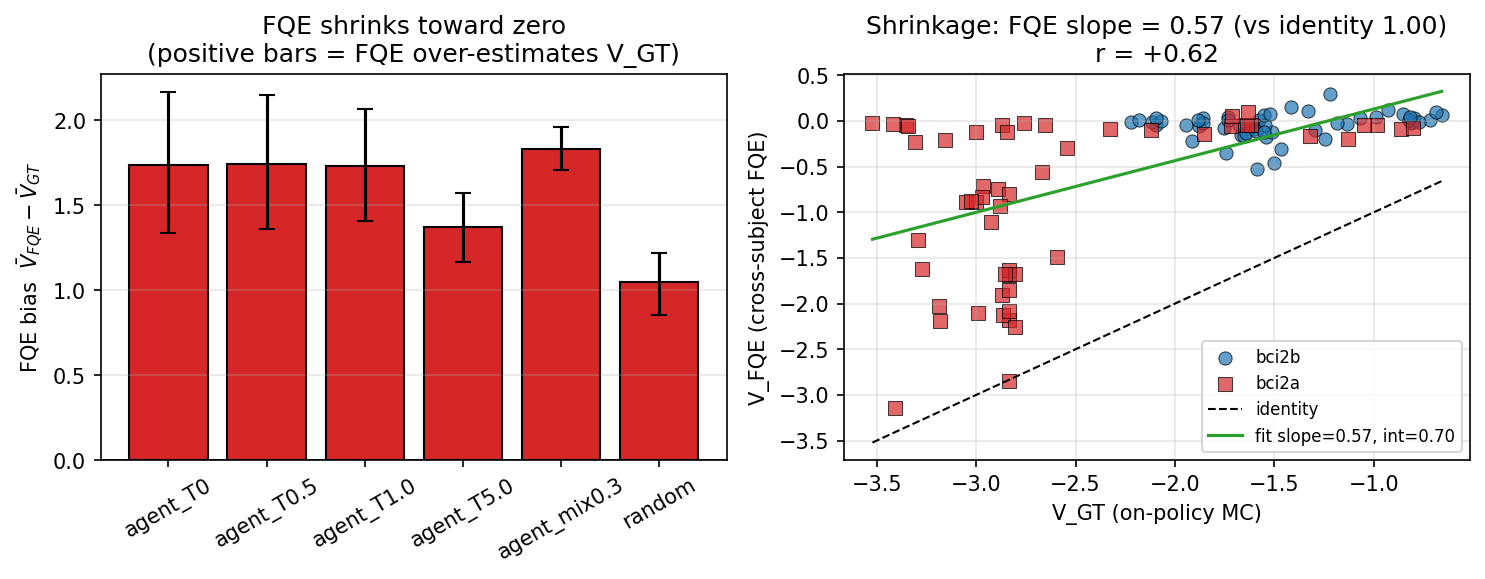
\includegraphics[width=\columnwidth]{../figures/fqe_bias_decomposition.png}
\caption{Fitted-Q estimator shrinks toward zero on the
$N\!=\!9$~LOSO OPE corpus. Linear fit
$V_{\fqe}\!=\!0.57\,V_{\text{GT}}\!+\!0.70$ ($r\!=\!+0.62$);
weak-decodability subjects (red) exhibit $44\%$ larger shrinkage.}
\label{fig:app:fqe_bias}
\end{figure}

\fqe{} shrinks toward zero
($V_{\fqe}\!=\!0.57\,V_{\text{GT}}\!+\!0.70$, $r\!=\!+0.62$;
$44\%$ more on weak-decodability subjects, see
Fig.~\ref{fig:app:fqe_bias}). Any monotone affine
correction $\hat V = (V_{\fqe} - b)/m$ preserves within-subject
argmax over policies, so the LOSO-corrected $\Delta$ versus naive
\fqe{} on policy selection is identically zero ($+0.000$) on all 9
subjects. Subject-conditioning is therefore \emph{necessary} for any
OPE-bias correction to alter cross-subject policy selection.

% =========================================================================
\section{Hyperparameters}\label{app:hp}
% =========================================================================

\begin{table}[H]
\centering
\caption{Hyperparameters across all experiments unless noted.}
\label{tab:app:hp}
\footnotesize
\begin{tabular}{l l}
\toprule
Parameter & Value \\
\midrule
Window length $L$ / stride $\Delta$    & $1.0$~s / $0.25$~s \\
Reward $R^+ / R^- / R_a / R_{\text{recal}}$ & $+1$ / $-5$ / $-0.5$ / $-0.3$ \\
Time cost $\lambda$                     & $0.05$~s$^{-1}$ \\
EEGNet $F_1$, $D$ / params              & $8$, $2$ / $\sim$1.5K \\
EEGNet pretrain epochs / lr / wd        & $20$ / $10^{-3}$ / $10^{-4}$ \\
LaBraM params / fine-tune epochs / lr   & $5.8$M / $8$ / $10^{-4}$ \\
EEG-Conformer emb / depth / heads / drop & $40$ / $6$ / $10$ / $0.5$ \\
EEG-Conformer epochs / lr / $\beta_1$   & $80$ / $2\!\times\!10^{-4}$ / $0.5$ \\
Q-net hidden / depth                    & $256$ / $3$ \\
\cql{} $\alpha$ / CVaR $\alpha_{\cvar}$ & $1.0$ / $0.25$ \\
CMDP $\epsilon$ / dual-lr               & $0.10$ / $5\!\times\!10^{-3}$ \\
$\gamma$ / Polyak $\tau$                & $0.99$ / $5\!\times\!10^{-3}$ \\
Gradient steps (within / LOSO)          & $20$K / $10$K \\
Batch size                              & $256$ \\
FQE Bellman iters / Bootstrap $B$       & $500$ / $10{,}000$ \\
\bottomrule
\end{tabular}
\end{table}

% =========================================================================
\section{Reproducibility}\label{app:repro}
% =========================================================================

\textbf{Hardware}: NVIDIA RTX 3080 (10 GB), CUDA 12.4;
$\sim\!24$ GPU-hours total.
\textbf{Software}: Python 3.11, PyTorch 2.6, MNE, MOABB,
braindecode 0.9, d3rlpy, scikit-learn.
\textbf{Datasets} (public, via MOABB): \bcib{}
(\texttt{BNCI2014\_004}), \bcia{} (\texttt{BNCI2014\_001}), Lee2019
(\texttt{Lee2019\_MI}). All $\pm$ values are over 5 seeds; data
preprocessing is deterministic.
\textbf{Code} (anonymised, de-anonymised under MIT at
camera-ready): pipeline + per-experiment summary JSONs at
\url{https://anonymous.4open.science/r/NeuroPolicy-AFB8}; every
claim traces to a JSON in \texttt{experiments/}.

\end{document}
